\documentclass{article} % A4 paper and 11pt font size
\setcounter{secnumdepth}{0}

\usepackage{amssymb, amsmath, amsfonts}
\usepackage{moreverb}
\usepackage{graphicx}
\usepackage{enumerate}
\usepackage{caption}
\usepackage{graphics}
\usepackage[margin=1in]{geometry}
\usepackage{color}
\usepackage{tocloft}
\renewcommand{\cftsecleader}{\cftdotfill{\cftdotsep}}
\usepackage{array}
\usepackage{arydshln}
\usepackage{float}
\usepackage{csquotes}
\usepackage{placeins}
\usepackage{verbatim}
\usepackage{hyperref}
\usepackage{textcomp}
\usepackage[makeroom]{cancel}
\usepackage{bbold}
\usepackage{scrextend}
\usepackage{alltt}
\usepackage{listings}
\usepackage{physics}
\usepackage{mathtools}
\usepackage[normalem]{ulem}
\usepackage{amsthm}
\usepackage{tikz}
\usetikzlibrary{positioning}
\usetikzlibrary{arrows}
\usepackage{pgfplots}
\usepackage{bigints}
\allowdisplaybreaks
\pgfplotsset{compat=1.12}

\theoremstyle{plain}
\newtheorem*{theorem*}{Theorem}
\newtheorem{theorem}{Theorem}
\newtheorem*{lemma*}{Lemma}
\newtheorem{lemma}{Lemma}

\definecolor{verbgray}{gray}{0.9}
% \definecolor{dkgreen}{green}{0.9}

\lstnewenvironment{code}{%
  \lstset{
  language=Python,
  backgroundcolor=\color{verbgray},
  keywordstyle=\color{blue},      % keyword style
  keywordstyle=[2]\color{blue},   % keyword style
  commentstyle=\color{magenta},   % comment style
  stringstyle=\color{olive},      % string literal styleframe=single,
  numberstyle=\color{black},      % string literal styleframe=single,
  framerule=0pt,
  numbers=left,
  stepnumber=1,
  firstnumber=1,
  showspaces=false,
  basicstyle=\ttfamily}}{}

\lstnewenvironment{console_output}{%
  \lstset{
  framerule=0pt,
  numbers=left,
  stepnumber=1,
  showspaces=false,
  firstnumber=1,
  basicstyle=\ttfamily}}{}


\makeatletter
\newcommand{\BIGG}{\bBigg@{3}}
\newcommand{\vast}{\bBigg@{4}}
\newcommand{\Vast}{\bBigg@{5}}
\makeatother

\newenvironment{definition}[1][Definition]{\begin{trivlist}
\item[\hskip \labelsep {\bfseries #1}]}{\end{trivlist}}

\newcommand{\dy}{\partial_y}
\newcommand{\dyy}{\partial_{yy}}
\newcommand{\dxx}{\partial_{xx}}
\newcommand{\dxy}{\partial_{xy}}
\newcommand{\dyyy}{\partial_{yyy}}
\newcommand{\dxxx}{\partial_{xxx}}
\newcommand{\dx}{\partial_x}
\newcommand{\E}{\varepsilon}
\def\Rl{\mathbb{R}}
\def\Cx{\mathbb{C}}

\newcommand{\Ei}{\text{Ei}}

\usepackage[T1]{fontenc} % Use 8-bit encoding that has 256 glyphs
\usepackage{fourier} % Use the Adobe Utopia font for the document - comment this line to return to the LaTeX default
\usepackage[english]{babel} % English language/hyphenation

\usepackage{sectsty} % Allows customizing section commands
\allsectionsfont{\centering \normalfont\scshape} % Make all sections centered, the default font and small caps

\usepackage{fancyhdr} % Custom headers and footers
\pagestyle{fancy} % Makes all pages in the document conform to the custom headers and footers
\fancyhead[L]{\bf Sam Fleischer}
\fancyhead[C]{\bf UC Davis \\ Numerical Solutions of Differential Equations (MAT228A)} % No page header - if you want one, create it in the same way as the footers below
\fancyhead[R]{\bf Fall 2016}

\fancyfoot[L]{\bf } % Empty left footer
\fancyfoot[C]{\bf \thepage} % Empty center footer
\fancyfoot[R]{\bf } % Page numbering for right footer
\renewcommand{\headrulewidth}{0pt} % Remove header underlines
\renewcommand{\footrulewidth}{0pt} % Remove footer underlines
\setlength{\headheight}{25pt} % Customize the height of the header

\newcommand{\VEC}[2]{\left\langle #1, #2 \right\rangle}
\newcommand{\ran}{\text{\rm ran }}
\newcommand{\Hilb}{\mathcal{H}}
\newcommand{\lap}{\Delta}

\newcommand{\littleo}[1]{\text{\scriptsize$\mathcal{O}$}\qty(#1)}

\DeclareMathOperator*{\esssup}{\text{ess~sup}}

\newcommand{\problem}[2]{
\vspace{.375cm}
\boxed{\begin{minipage}{\textwidth}
    \section{\bf #1}
    #2
\end{minipage}}
}

\numberwithin{equation}{section} % Number equations within sections (i.e. 1.1, 1.2, 2.1, 2.2 instead of 1, 2, 3, 4)
\numberwithin{figure}{section} % Number figures within sections (i.e. 1.1, 1.2, 2.1, 2.2 instead of 1, 2, 3, 4)
\numberwithin{table}{section} % Number tables within sections (i.e. 1.1, 1.2, 2.1, 2.2 instead of 1, 2, 3, 4)

\setlength\parindent{0pt} % Removes all indentation from paragraphs - comment this line for an assignment with lots of text

\newcommand{\horrule}[1]{\rule{\linewidth}{#1}} % Create horizontal rule command with 1 argument of height

\title{ 
\normalfont \normalsize 
\textsc{UC Davis, Numerical Solutions of Differential Equations (MAT 228A), Fall 2016} \\ [25pt] % Your university, school and/or department name(s)
\horrule{2pt} \\[0.4cm] % Thin top horizontal rule
\Huge Homework \#2 \\ % The assignment title
\horrule{2pt} \\[0.5cm] % Thick bottom horizontal rule
}

\author{\huge Sam Fleischer} % Your name

\date{October 28, 2016} % Today's date or a custom date

\begin{document}\thispagestyle{empty}

\maketitle % Print the title

\makeatletter
\@starttoc{toc}
\makeatother

\pagebreak

%%%%%%%%%%%%%%%%%%%%%%%%%%%%%%%%%%%%%%
\problem{Problem 1}{Use the standard 3-point discretization of the Laplacian on a regular mesh to find a numerical solution to the PDEs below. Perform a refinement study using the exact solution to compute the error that shows the rate of convergence for both the 1-norm and the max norm.
\begin{enumerate}[\ \ (a)]
    \item $u_{xx} = \exp(x),\qquad u(0) = 0, \qquad u(1) = 1$
    \item $u_{xx} = 2\cos^2(\pi x),\qquad u_x(0) = 0, \qquad u_x(1) = 1$
\end{enumerate}
}
\begin{enumerate}[\ \ (a)]
    \item
        The discretization for $u_{xx} = f$ with Dirichlet boundary conditions $u(0) = \alpha$ and $u(1) = \beta$ is $A\vec{u} = \vec{b}$ where $A$ is an $N\times N$ matrix of the interior points (this does not include $0$ and $1$).
        \begin{align}
            A = \qty(\begin{array}{cccccc}
                -2 & 1 & 0 & \dots & \dots & 0 \\
                1 & -2 & 1 & 0 & \dots & 0 \\
                0 & 1 & -2 & 1 & \dots & 0 \\
                \vdots & \vdots & \ddots & \ddots & \ddots & \vdots \\
                0 & 0 & \dots & 1 & -2 & 1 \\
                0 & 0 & \dots & 0 & 1 & -2
            \end{array}) \qquad \text{and} \qquad \vec{b} = \qty(\begin{array}{c}
                f_1 - \frac{\alpha}{h^2} \\ f_2 \\ \vdots \\ f_{N-1} \\ f_N - \frac{\beta}{h^2}
            \end{array}).
        \end{align}
        $A$ is invertible, and so we can directly solve for $\vec{u}$ by $\vec{u} = A^{-1}\vec{b}$.  In Python I used the fact that $A$ is sparse to speed up the calculations.  The exact solution is
        \begin{align}
            u(x) = e^x + (2 - e)x - 1
        \end{align}
        The following is the code I used to generate the graphs.
        \begin{code}
def solution(x):
    return np.exp(x) + (2 - math.exp(1))*x - 1

def one_norm_error(a,b,h):
    S = 0
    for i in range(len(a)):
        S += abs(a[i]-b[i])
    return S*h

def max_norm_error(a,b):
    S = 0
    for i in range(len(a)):
        S = max(S, abs(a[i]-b[i]))
    return S

one = []
Max = []

Ns = [10*i for i in range(1,100)]

for N in Ns:
    h = 1/(1 + N)
    sub_diag = 1/(h**2)*np.ones(N)
    super_diag = 1/(h**2)*np.ones(N)
    diag = -2/(h**2)*np.ones(N)

    A = np.vstack((sub_diag,diag,super_diag))
    A = scipy.sparse.dia_matrix((A,[-1,0,1]),shape=(N,N))
    A = scipy.sparse.csc_matrix(A)

    grid_pts = np.linspace(h, 1-h, num=N)
    b = np.exp(grid_pts)
    b[-1] -= 1/(h**2)

    u = scipy.sparse.linalg.spsolve(A, b)

    tru_sol = solution(grid_pts)

    e_1 = one_norm_error(tru_sol,u,h)
    e_m = max_norm_error(tru_sol,u)

    one.append(e_1)
    Max.append(e_m)
        \end{code}
        Then I plotted the results and generated a table:
        \begin{figure}[ht!]
            \centering
            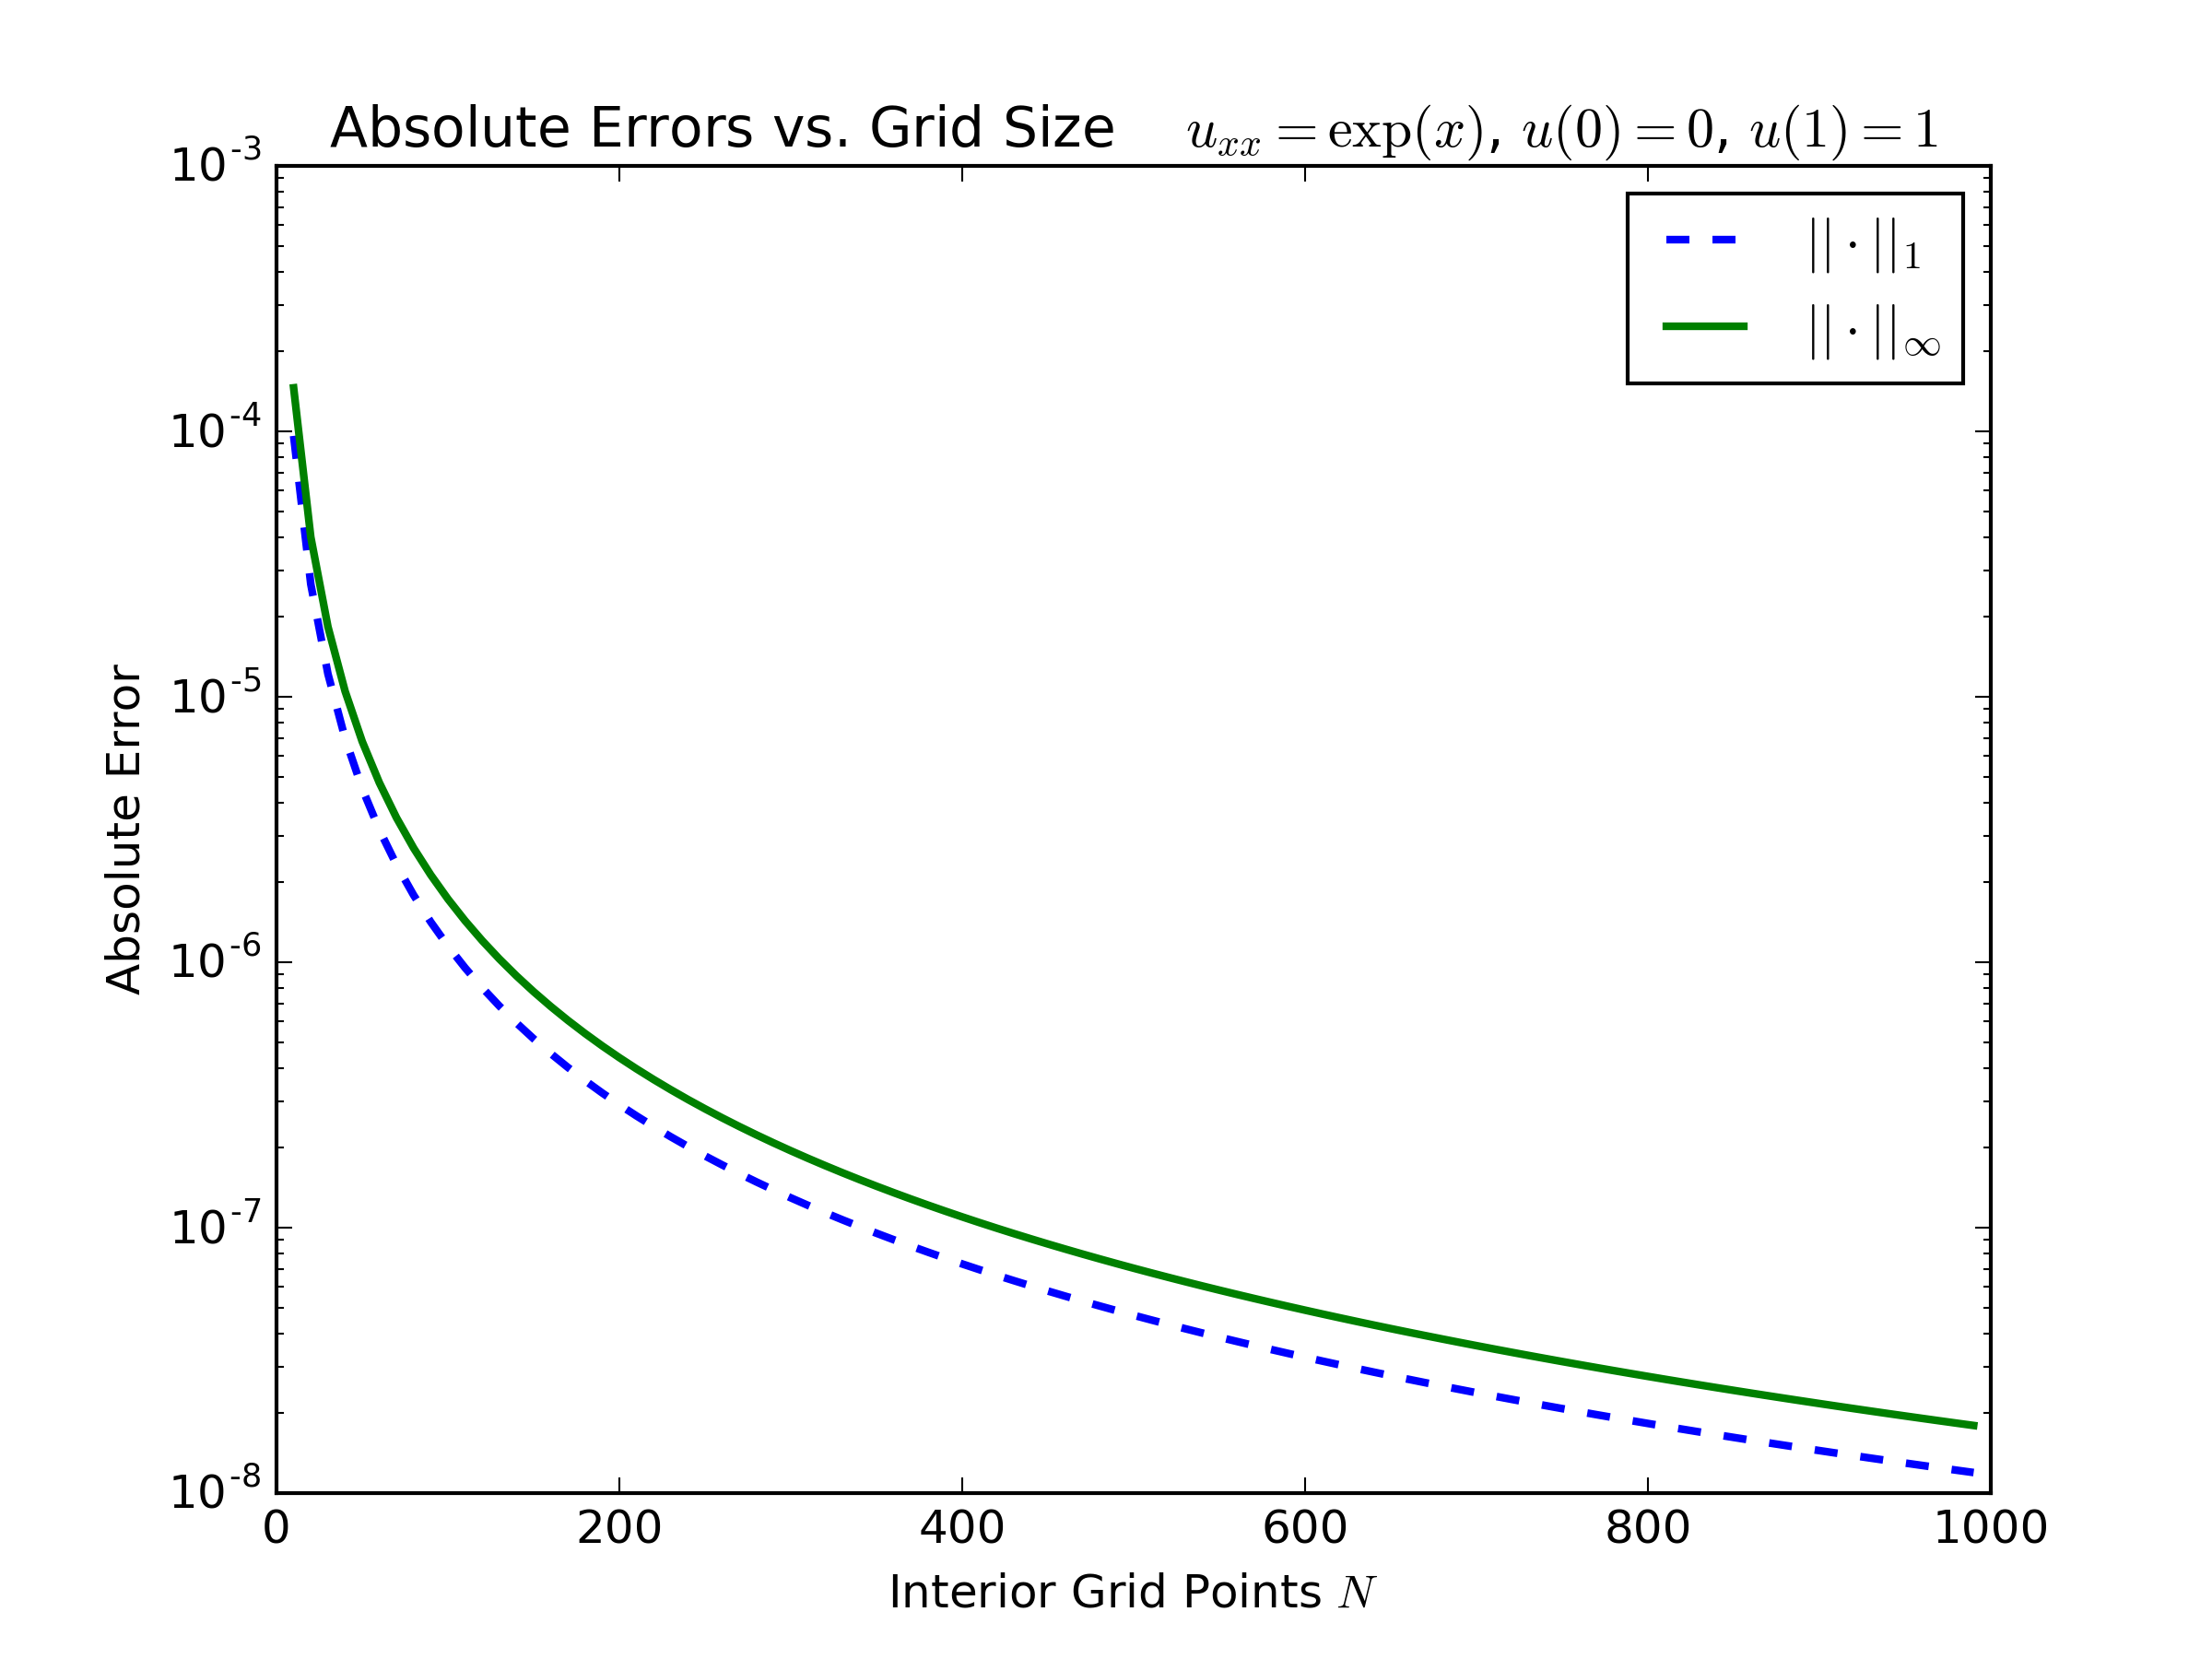
\includegraphics[scale=0.5]{figure_1a.png}
        \end{figure}
        \begin{center}
            \begin{tabular}[ht!]{lllll}
                \hline
                    $N$ &    $\norm{\cdot}_1$ errors &   $\norm{\cdot}_1$ ratios &    $\norm{\cdot}_\infty$ errors &   $\norm{\cdot}_\infty$ ratios \\
                \hline
                    2 & 0.00115081  &          -        & 0.00182123  &          -        \\
                    4 & 0.000449552 &          0.39064  & 0.000694778 &          0.381487 \\
                    8 & 0.00014301  &          0.318117 & 0.000217656 &          0.313274 \\
                   16 & 4.04669e-05 &          0.282966 & 6.10464e-05 &          0.280472 \\
                   32 & 1.07684e-05 &          0.266103 & 1.62108e-05 &          0.265549 \\
                   64 & 2.77758e-06 &          0.257939 & 4.17864e-06 &          0.25777  \\
                  128 & 7.05337e-07 &          0.253939 & 1.06096e-06 &          0.2539   \\
                  256 & 1.77718e-07 &          0.251961 & 2.6731e-07  &          0.251951 \\
                  512 & 4.46033e-08 &          0.250979 & 6.70883e-08 &          0.250976 \\
                 1024 & 1.11727e-08 &          0.250491 & 1.68049e-08 &          0.25049  \\
                \hline
            \end{tabular}
        \end{center}
        Notice I am doubling the grid size $N$ and both $\norm{\cdot}_1$ and $\norm{\cdot}_\infty$ errors are decreasing by a factor of $4$.  Thus this method is $\order{h^2}$.
    \item
        The discretization for $u_{xx} = f$ with Neumann boundary conditions $u_x(0) = \alpha$ and $u_x(1) = \beta$ is different than before.  We must first note that this operator is singular and thus $u_{xx} = f$ with these boundary conditios is only solvable if $f \in \ran L$ where $L = \frac{\partial^2}{\partial x^2}$ with these boundary conditions.  So first we must ensure that $2\cos^2(\pi x) \in \ran L$, which is trivially true.  However if $u$ is a solution of $u_{xx} = f$, it may not be a solution of a discritization $A\vec{u} = \vec{b}$.  Let $\vec{v}$ span $\ker[A]$.  Then $A\vec{u} = b - \lambda\vec{v}$ is solvable (where $\lambda$ is the coefficient of the projection $b$ on to $\ker[A]$).  Then we are solving
        \begin{align}
            A\vec{u} + \lambda\vec{v} = \vec{b}
        \end{align}
        which is an $(N+3)$ dimensional linear system where $N$ is the number of interior points, not including $0$ and $1$.  We must impose a condition on $\vec{u}$ in order to get another equation, for example, $\sum_i u_i = 0$.  This gives us the discritization $M\vec{q} = \vec{d}$ where
        \begin{align}
            M = \qty(\begin{array}{c;{2pt/2pt}c}
                A & \vec{v} \\ \hdashline[2pt/2pt] \vec{1}^T & 0
            \end{array}) \qquad \text{and} \qquad \vec{q} = \qty(\begin{array}{c}
                \vec{u} \\ \hdashline[2pt/2pt] \lambda
            \end{array}) \qquad \text{and} \qquad \vec{d} = \qty(\begin{array}{c} \vec{b} \\ \hdashline[2pt/2pt] 0\end{array})
        \end{align}
        where $\vec{v} = \qty(1\ \ \ 2\ \ \ 2\ \ \ \dots\ \ \ 2\ \ \ 1)^T$ and
        \begin{align}
            A = \qty(\begin{array}{cccccc}
                -2 & 2 & 0 & \dots & \dots & 0 \\
                1 & -2 & 1 & 0 & \dots & 0 \\
                0 & 1 & -2 & 1 & \dots & 0 \\
                \vdots & \vdots & \ddots & \ddots & \ddots & \vdots \\
                0 & 0 & \dots & 1 & -2 & 1 \\
                0 & 0 & \dots & 0 & 2 & -2
            \end{array}) \qquad \text{and} \qquad \vec{b} = \qty(\begin{array}{c}
                f_0 + \frac{2\alpha}{h} \\ f_2 \\ \vdots \\ f_{N-1} \\ f_{N+1} - \frac{\beta}{2h}
            \end{array}).
        \end{align}
        $M$ is invertible, and so we can directly solve for $\vec{q}$ by $\vec{q} = M^{-1}\vec{b}$.  Note that solving for $\vec{q}$ gives us $\vec{u}$.  Since, if $u$ is a solution to $u_{xx} = f$, then $u+C$ is also a solution for any constant $C$, I subtract the appropriate constant when comparing with any given discrete solution.  The following is the code I used to generate the graphs.
        \begin{code}
def solution(x,N):
    mean_zero_sol=0.5*(x**2)-(1/(4*(np.pi**2)))*np.cos(2*np.pi*x)-(1/6)
    sol = mean_zero_sol - (1/(N+2))*sum(mean_zero_sol)
    return sol

def one_norm_error(a,b,h):
    S = 0
    for i in range(len(a)):
        S += abs(a[i]-b[i])
    return S*h

def max_norm_error(a,b):
    S = 0
    for i in range(len(a)):
        S = max(S, abs(a[i]-b[i]))
    return S

one = []
Max = []

Ns = [10*i for i in range(1,100)]

for N in Ns:
    h = 1/(1 + N)

    sub_diag = np.concatenate((1/(h**2)*np.ones(N), [2/(h**2),0]))
    super_diag = np.concatenate(([0,2/(h**2)], 1/(h**2)*np.ones(N)))
    diag = -2/(h**2)*np.ones(N+2)

    v = np.append([1], np.append(2*np.ones((N,1)),[1]))
    A = np.vstack((sub_diag,diag,super_diag))
    A = scipy.sparse.dia_matrix((A,[-1,0,1]),shape=(N+2,N+2))
    A = scipy.sparse.hstack([A, v.reshape(N+2,1)])
    A = scipy.sparse.vstack([A, np.concatenate((np.ones(N+2),[0]))])
    A = scipy.sparse.csc_matrix(A)

    grid_pts = np.linspace(0, 1, num=(N+2))
    b = 2*(np.cos(np.pi*grid_pts)**2)
    b[-1] = b[-1] - (2/h)

    u = scipy.sparse.linalg.spsolve(A, np.concatenate((b, [0])))
    u = np.delete(u,N+2)

    tru_sol = solution(grid_pts, N)

    e_1 = one_norm_error(tru_sol,u,h)
    e_m = max_norm_error(tru_sol,u)

    one.append(e_1)
    Max.append(e_m)
        \end{code}
        Then I plotted the results and generated a table:
        \begin{figure}[ht!]
            \centering
            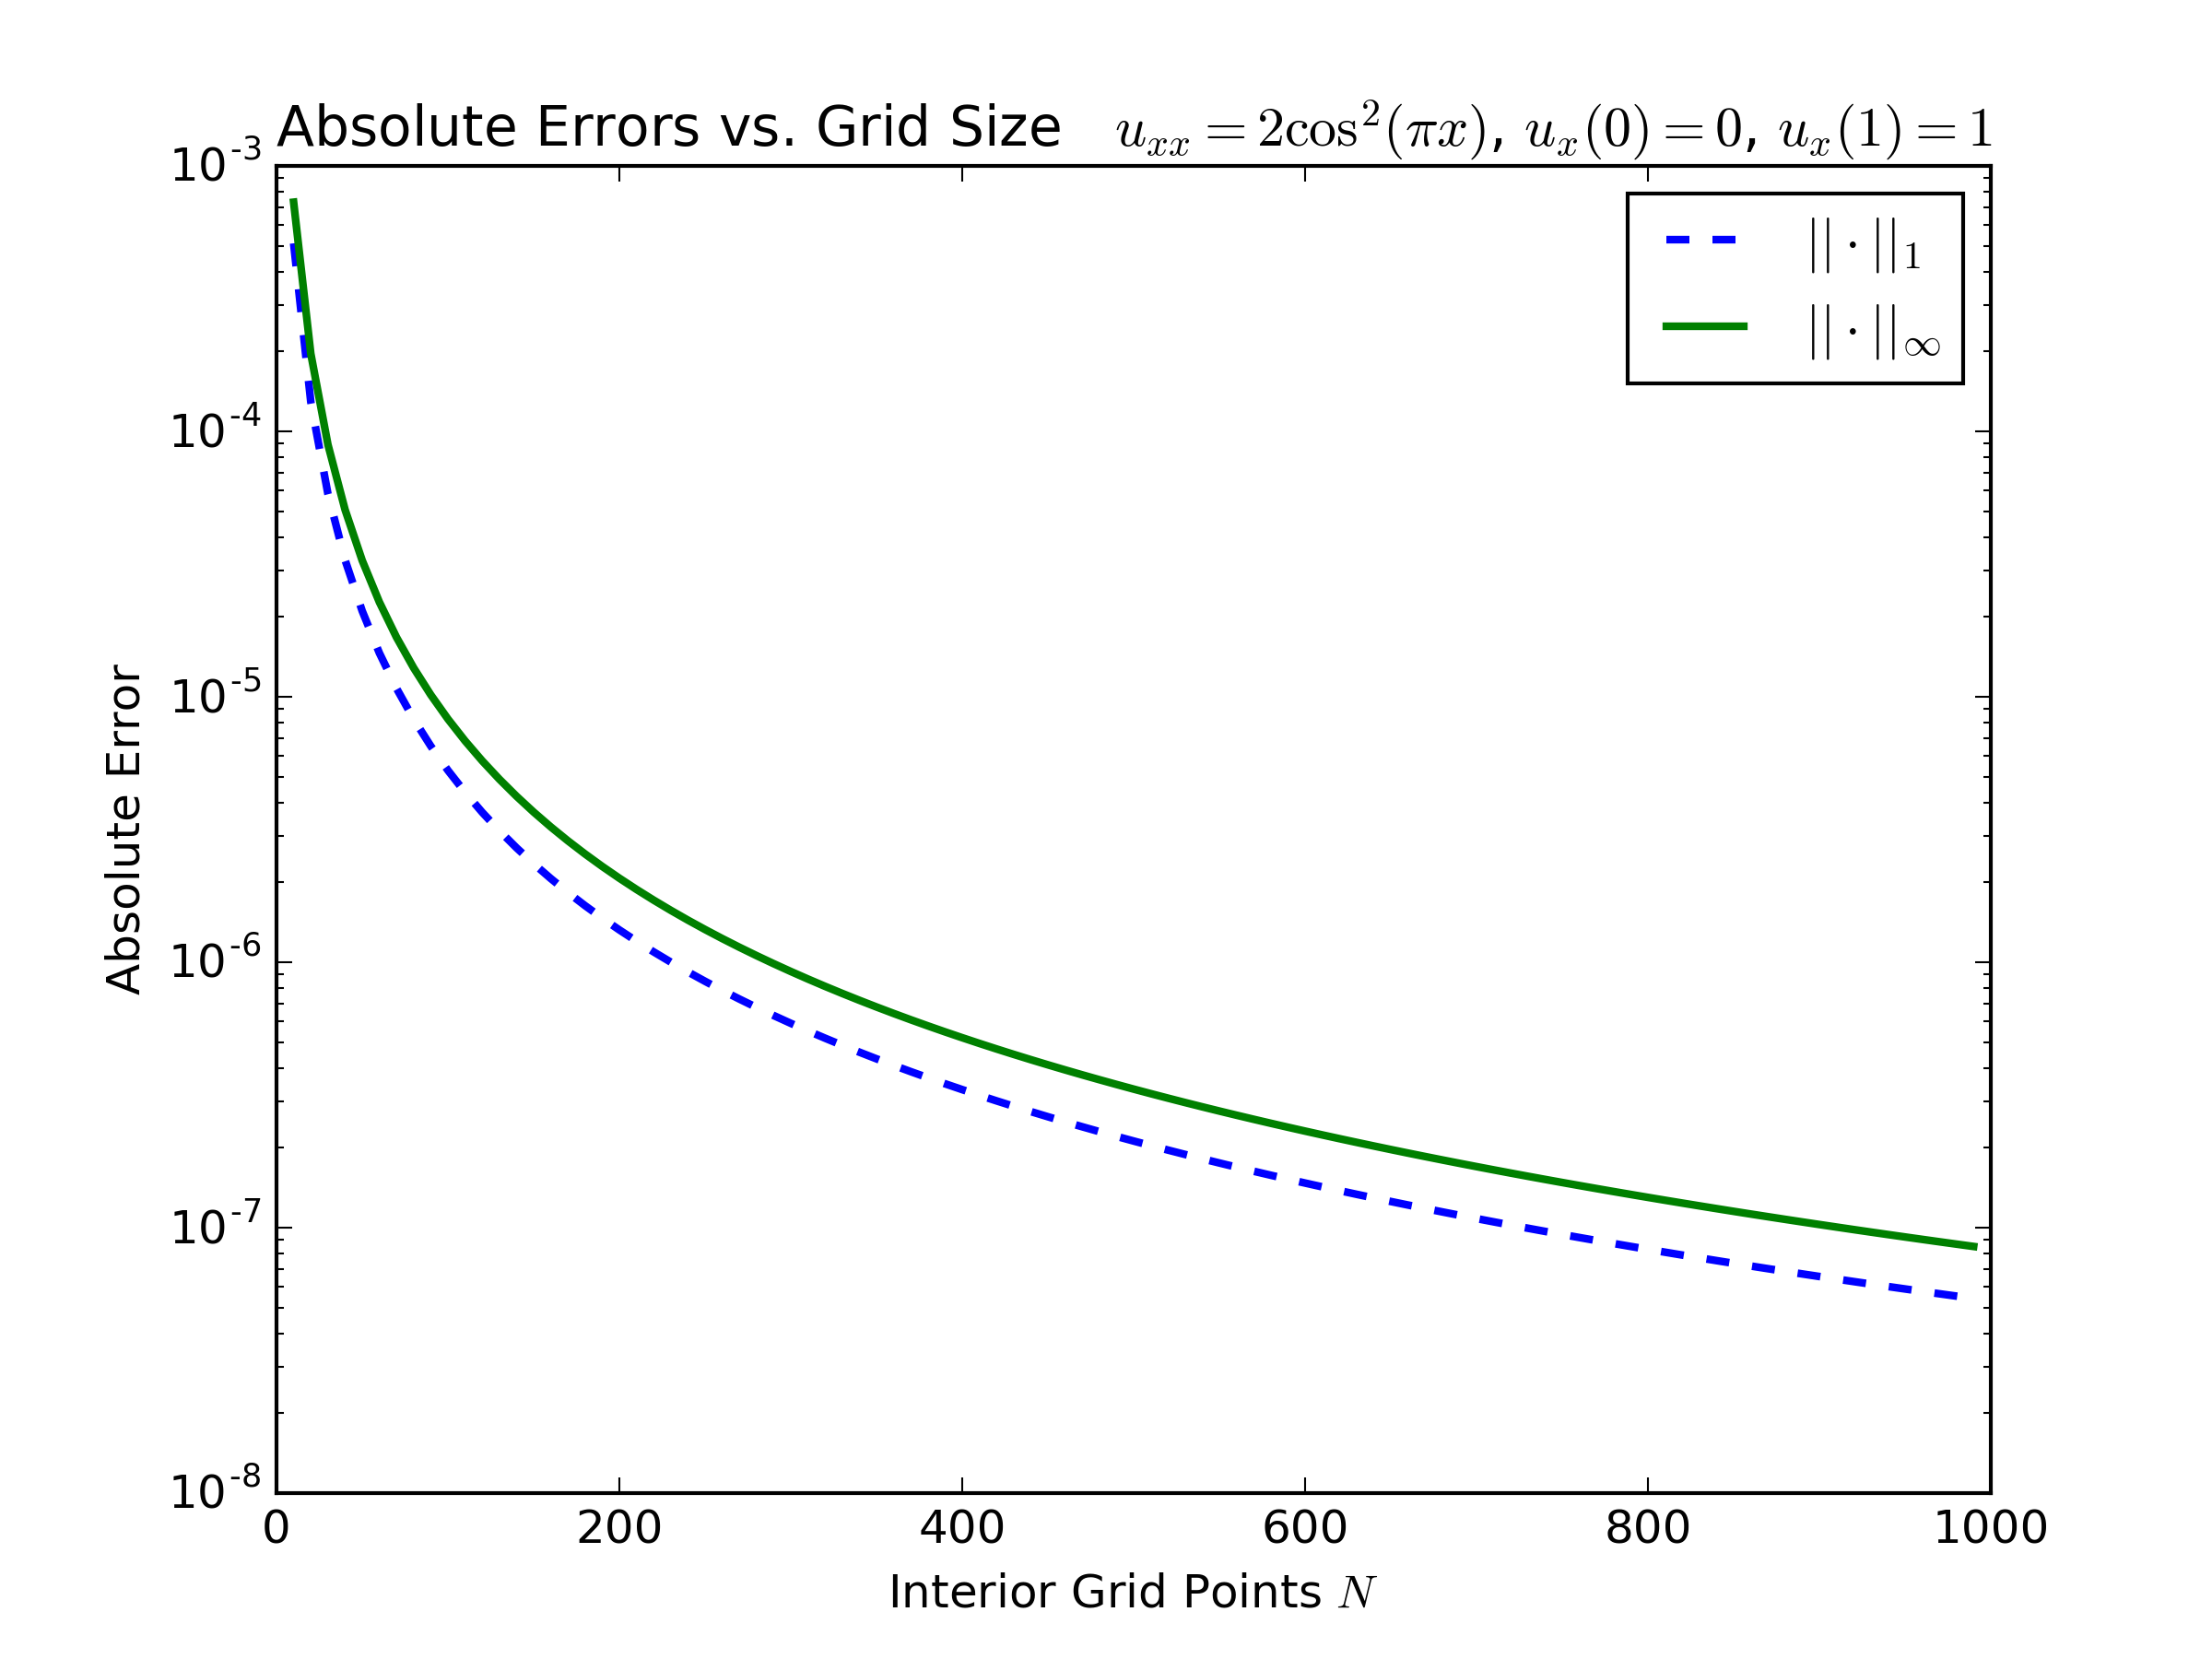
\includegraphics[scale=0.5]{figure_1b.png}
        \end{figure}
        \begin{center}
            \begin{tabular}[ht!]{lllll}
                \hline
                    $N$ &    $\norm{\cdot}_1$ errors &   $\norm{\cdot}_1$ ratios &    $\norm{\cdot}_\infty$ errors &   $\norm{\cdot}_\infty$ ratios \\
                \hline
                    2 & 0.0117067   &          0        & 0.00878006  &          0        \\
                    4 & 0.00282088  &          0.240962 & 0.0035261   &          0.401603 \\
                    8 & 0.000768375 &          0.272389 & 0.00109622  &          0.310888 \\
                   16 & 0.000200274 &          0.260646 & 0.000301517 &          0.275051 \\
                   32 & 5.10092e-05 &          0.254697 & 7.85693e-05 &          0.26058  \\
                   64 & 1.28581e-05 &          0.252074 & 2.0009e-05  &          0.254667 \\
                  128 & 3.22669e-06 &          0.250947 & 5.04535e-06 &          0.252154 \\
                  256 & 8.08117e-07 &          0.250447 & 1.26652e-06 &          0.251028 \\
                  512 & 2.02204e-07 &          0.250217 & 3.17266e-07 &          0.250501 \\
                 1024 & 5.05727e-08 &          0.250107 & 7.9395e-08  &          0.250247 \\
                \hline
            \end{tabular}
        \end{center}
        Again, notice I am doubling the grid size $N$ and both $\norm{\cdot}_1$ and $\norm{\cdot}_\infty$ errors are decreasing by a factor of $4$.  Thus this method is $\order{h^2}$.

\end{enumerate}







\FloatBarrier
\pagebreak
%%%%%%%%%%%%%%%%%%%%%%%%%%%%%%%%%%%%%%
\problem{Problem 2}{As a general rule, we usually think that an $\order{h^p}$ local truncation error (LTE) leads to an $\order{h^p}$ error. However, in some cases the LTE can be lower order at some points without lowering the order of the error. Consider the standard second-order discretization of the Poisson equation on $[0, 1]$ with homogeneous boundary conditions. The standard discretization of this problem gives an $\order{h^p}$ LTE provided the the solution is at least $C^4$ . The LTE may be lower order because the solution is not $C^4$ or because we use a lower order discretization at some points.
\begin{enumerate}[\ \ (a)]
    \item Suppose that the LTE is $\order{h^p}$ at the first grid point ($x_1 = h$).  What effect does this have on the error?  What is the smallest value of $p$ that gives a second order accurate error?  Hint: Use equation (2.46) From LeVeque to aid in your argument.
    \item Suppose that the LTE is $\order{h^p}$ at an interior point (i.e.~a point that does not limit to the boundary as $h \rightarrow 0$).  What effect does this have on the error?  What is the smallest value of $p$ that gives a second order accurate error?
    \item Verify the results of your analysis from parts (a) and (b) using numerical tests.
\end{enumerate}}
\FloatBarrier

\begin{enumerate}[\ \ (a)]
    \item
        The Green's function is
        \begin{align}
            B_{ij} = \begin{cases}
                h(x_j - 1)x_i & \text{ if } i = 1,2,\dots, j \\
                h(x_i - 1)x_j & \text{ if } i = j+1,\dots, N
            \end{cases} = \begin{cases}
                ijh^3 - ih^2 & \text{ if } i = 1,2,\dots, j \\
                ijh^3 - jh^2 & \text{ if } i = j+1,\dots, N
            \end{cases}
        \end{align}
        where $x_i = ih$ and $x_j = jh$.  Near the exterior, for example at $j = 1$, the maximum of $B$ is a constant multiple of $h^2$, and thus is $\order{h^2}$.  Thus even truncation error of $h^p$ where $p = 0$ doesn't affect the $\order{h^2}$ convergence of the solution.
    \item
        Near the interior, on the other hand, for example at $j = \frac{N}{2}$, the maximum of $B$ is the $\frac{N}{2}$nd term in the column, which is $N^2h^3 - Nh = \order{h}$.  Thus, truncation error of $h^p$ where $p = 0$ affects the $\order{h^2}$ convergence of the solution by a factor of $h$.  For all $p \geq 1$, however, the rate of convergence is unaffected.
    \item
        The following are plots and table generated by similar Python code to problem 1.  Notice for an exterior point, $p \geq 0$ produces $\order{h^2}$ error, but $p = -1$ produces $\order{h}$ error.  For an interior point, $p \geq 1$ produces $\order{h^2}$ error, $p = 0$ produces $\order{h}$ error, and $p = -1$ doesn't allow for convergence at all.
        \begin{figure}[ht!]
            \begin{minipage}[b]{0.5\linewidth}
                \centering
                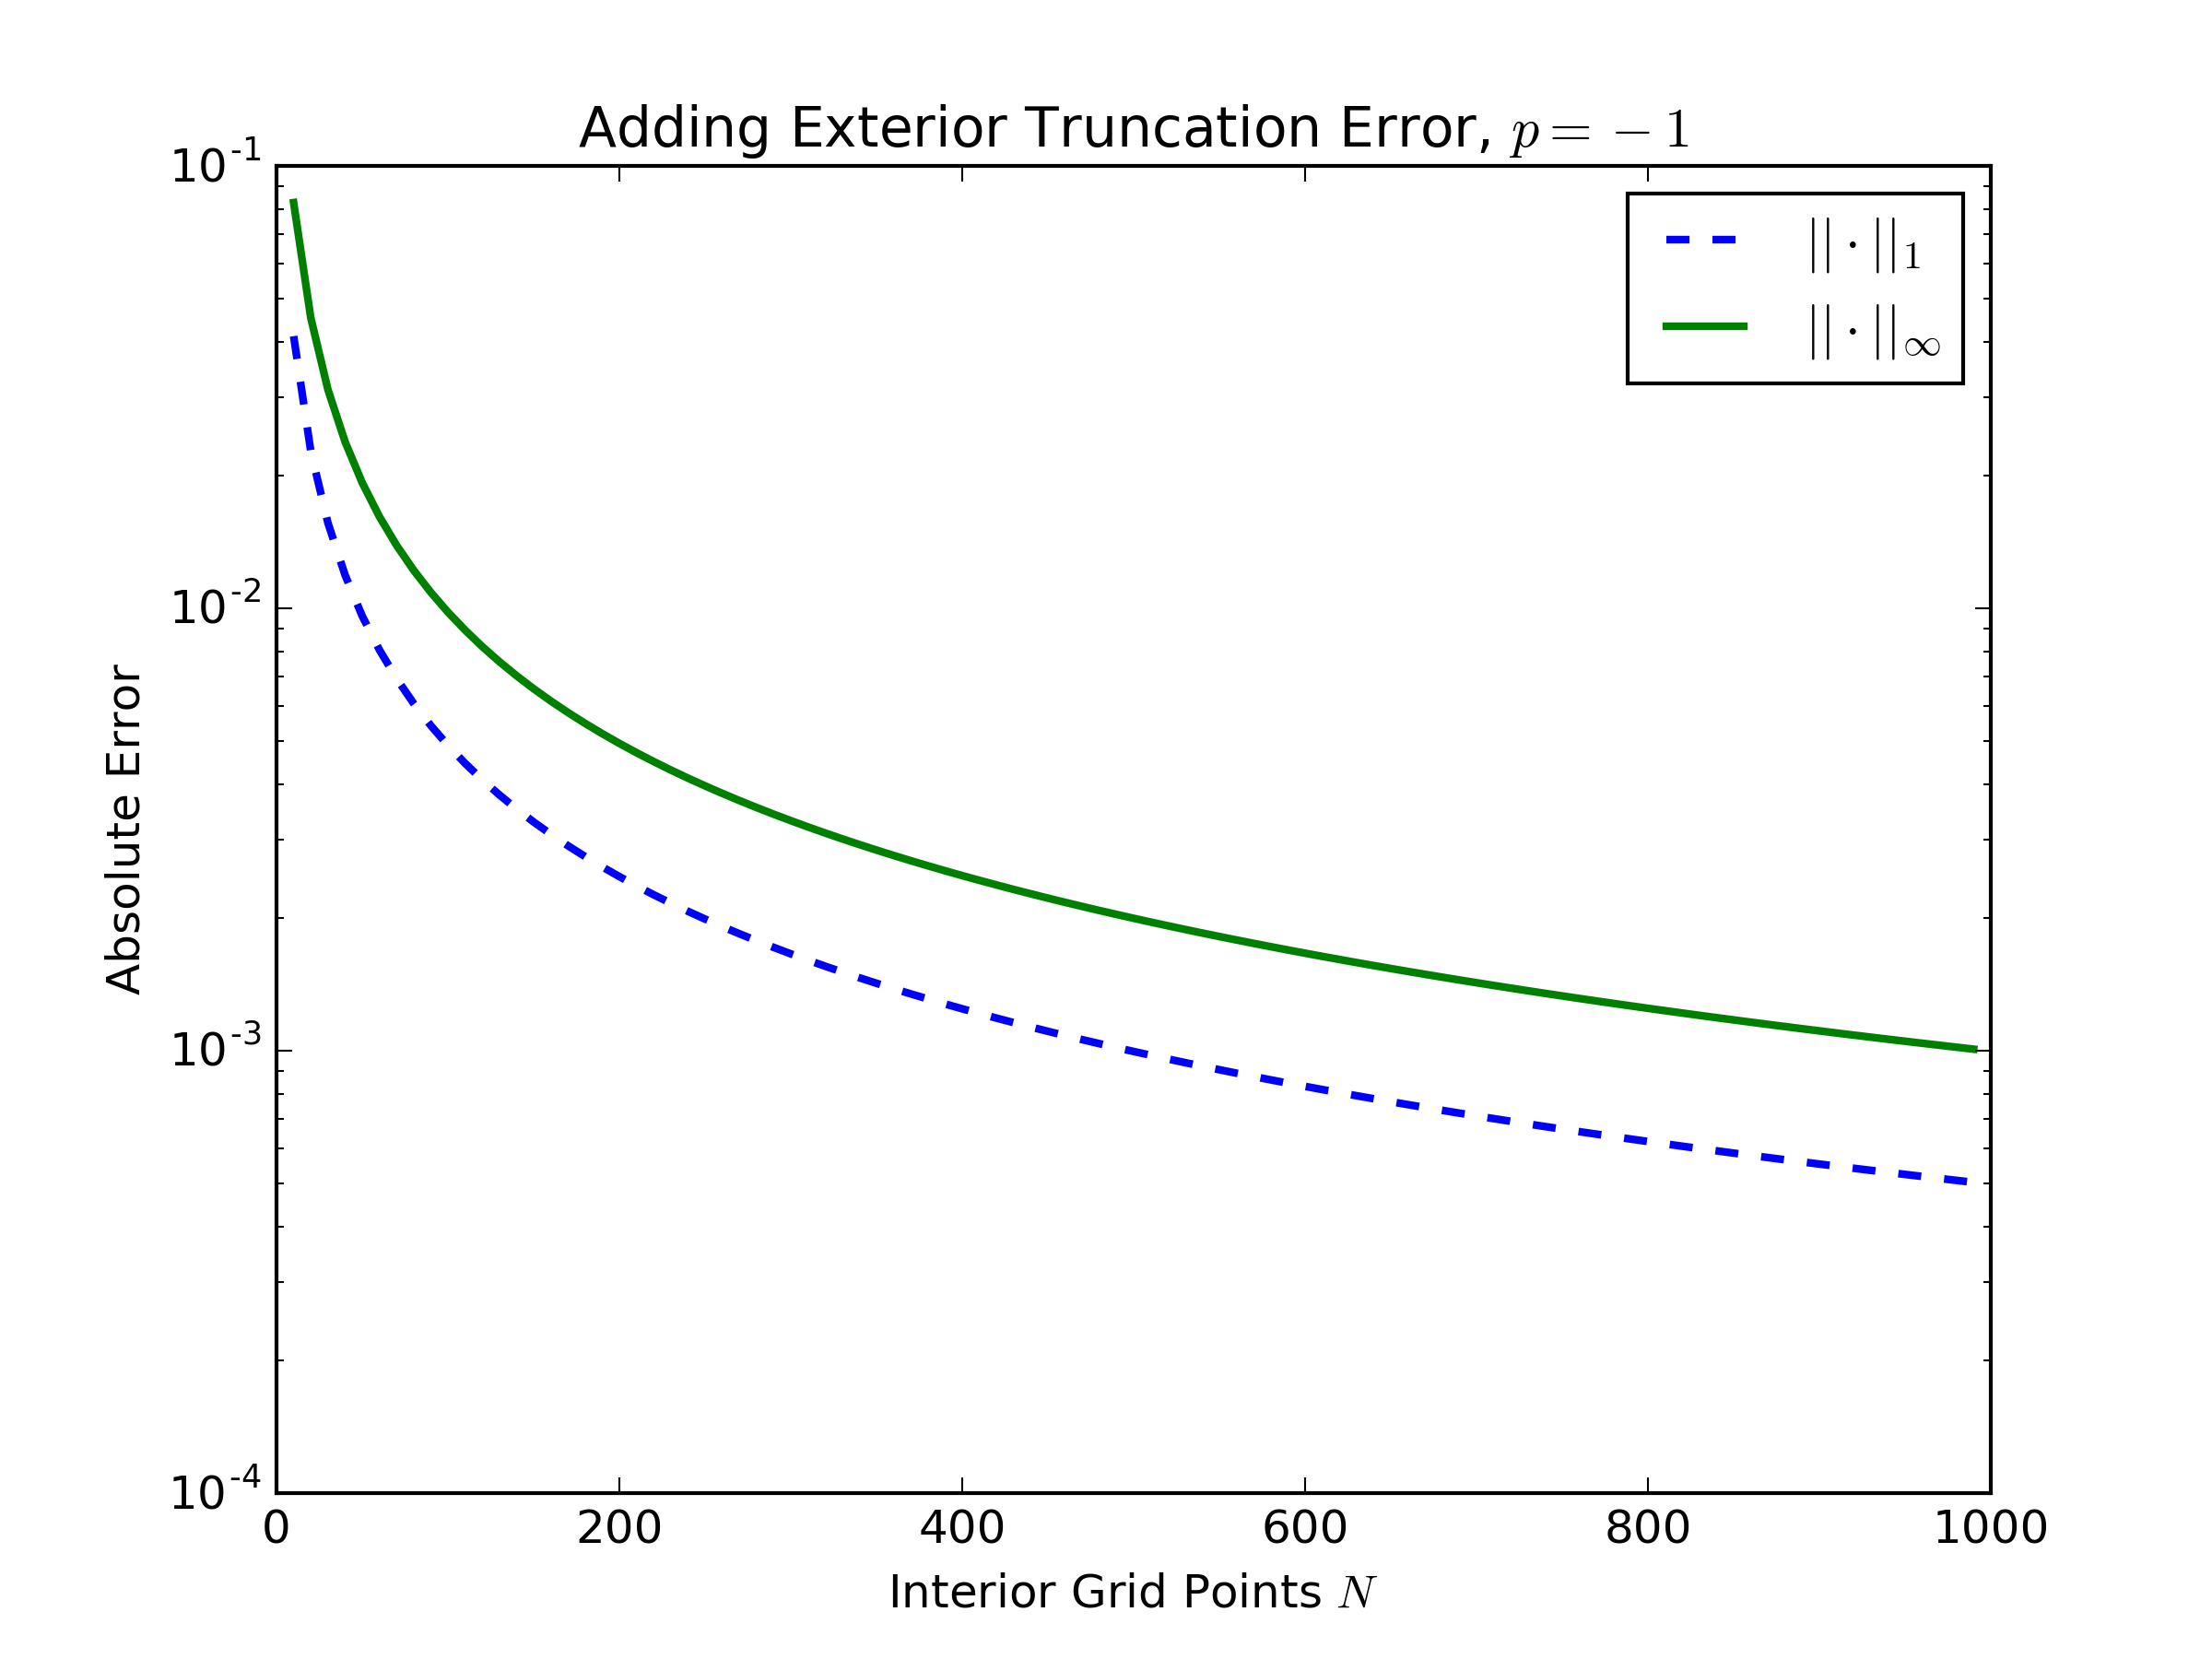
\includegraphics[width=\linewidth]{figure_2c1_ext_p=-1.png}
                \vspace{4ex}
            \end{minipage}%%
            \begin{minipage}[b]{0.5\linewidth}
                \centering
                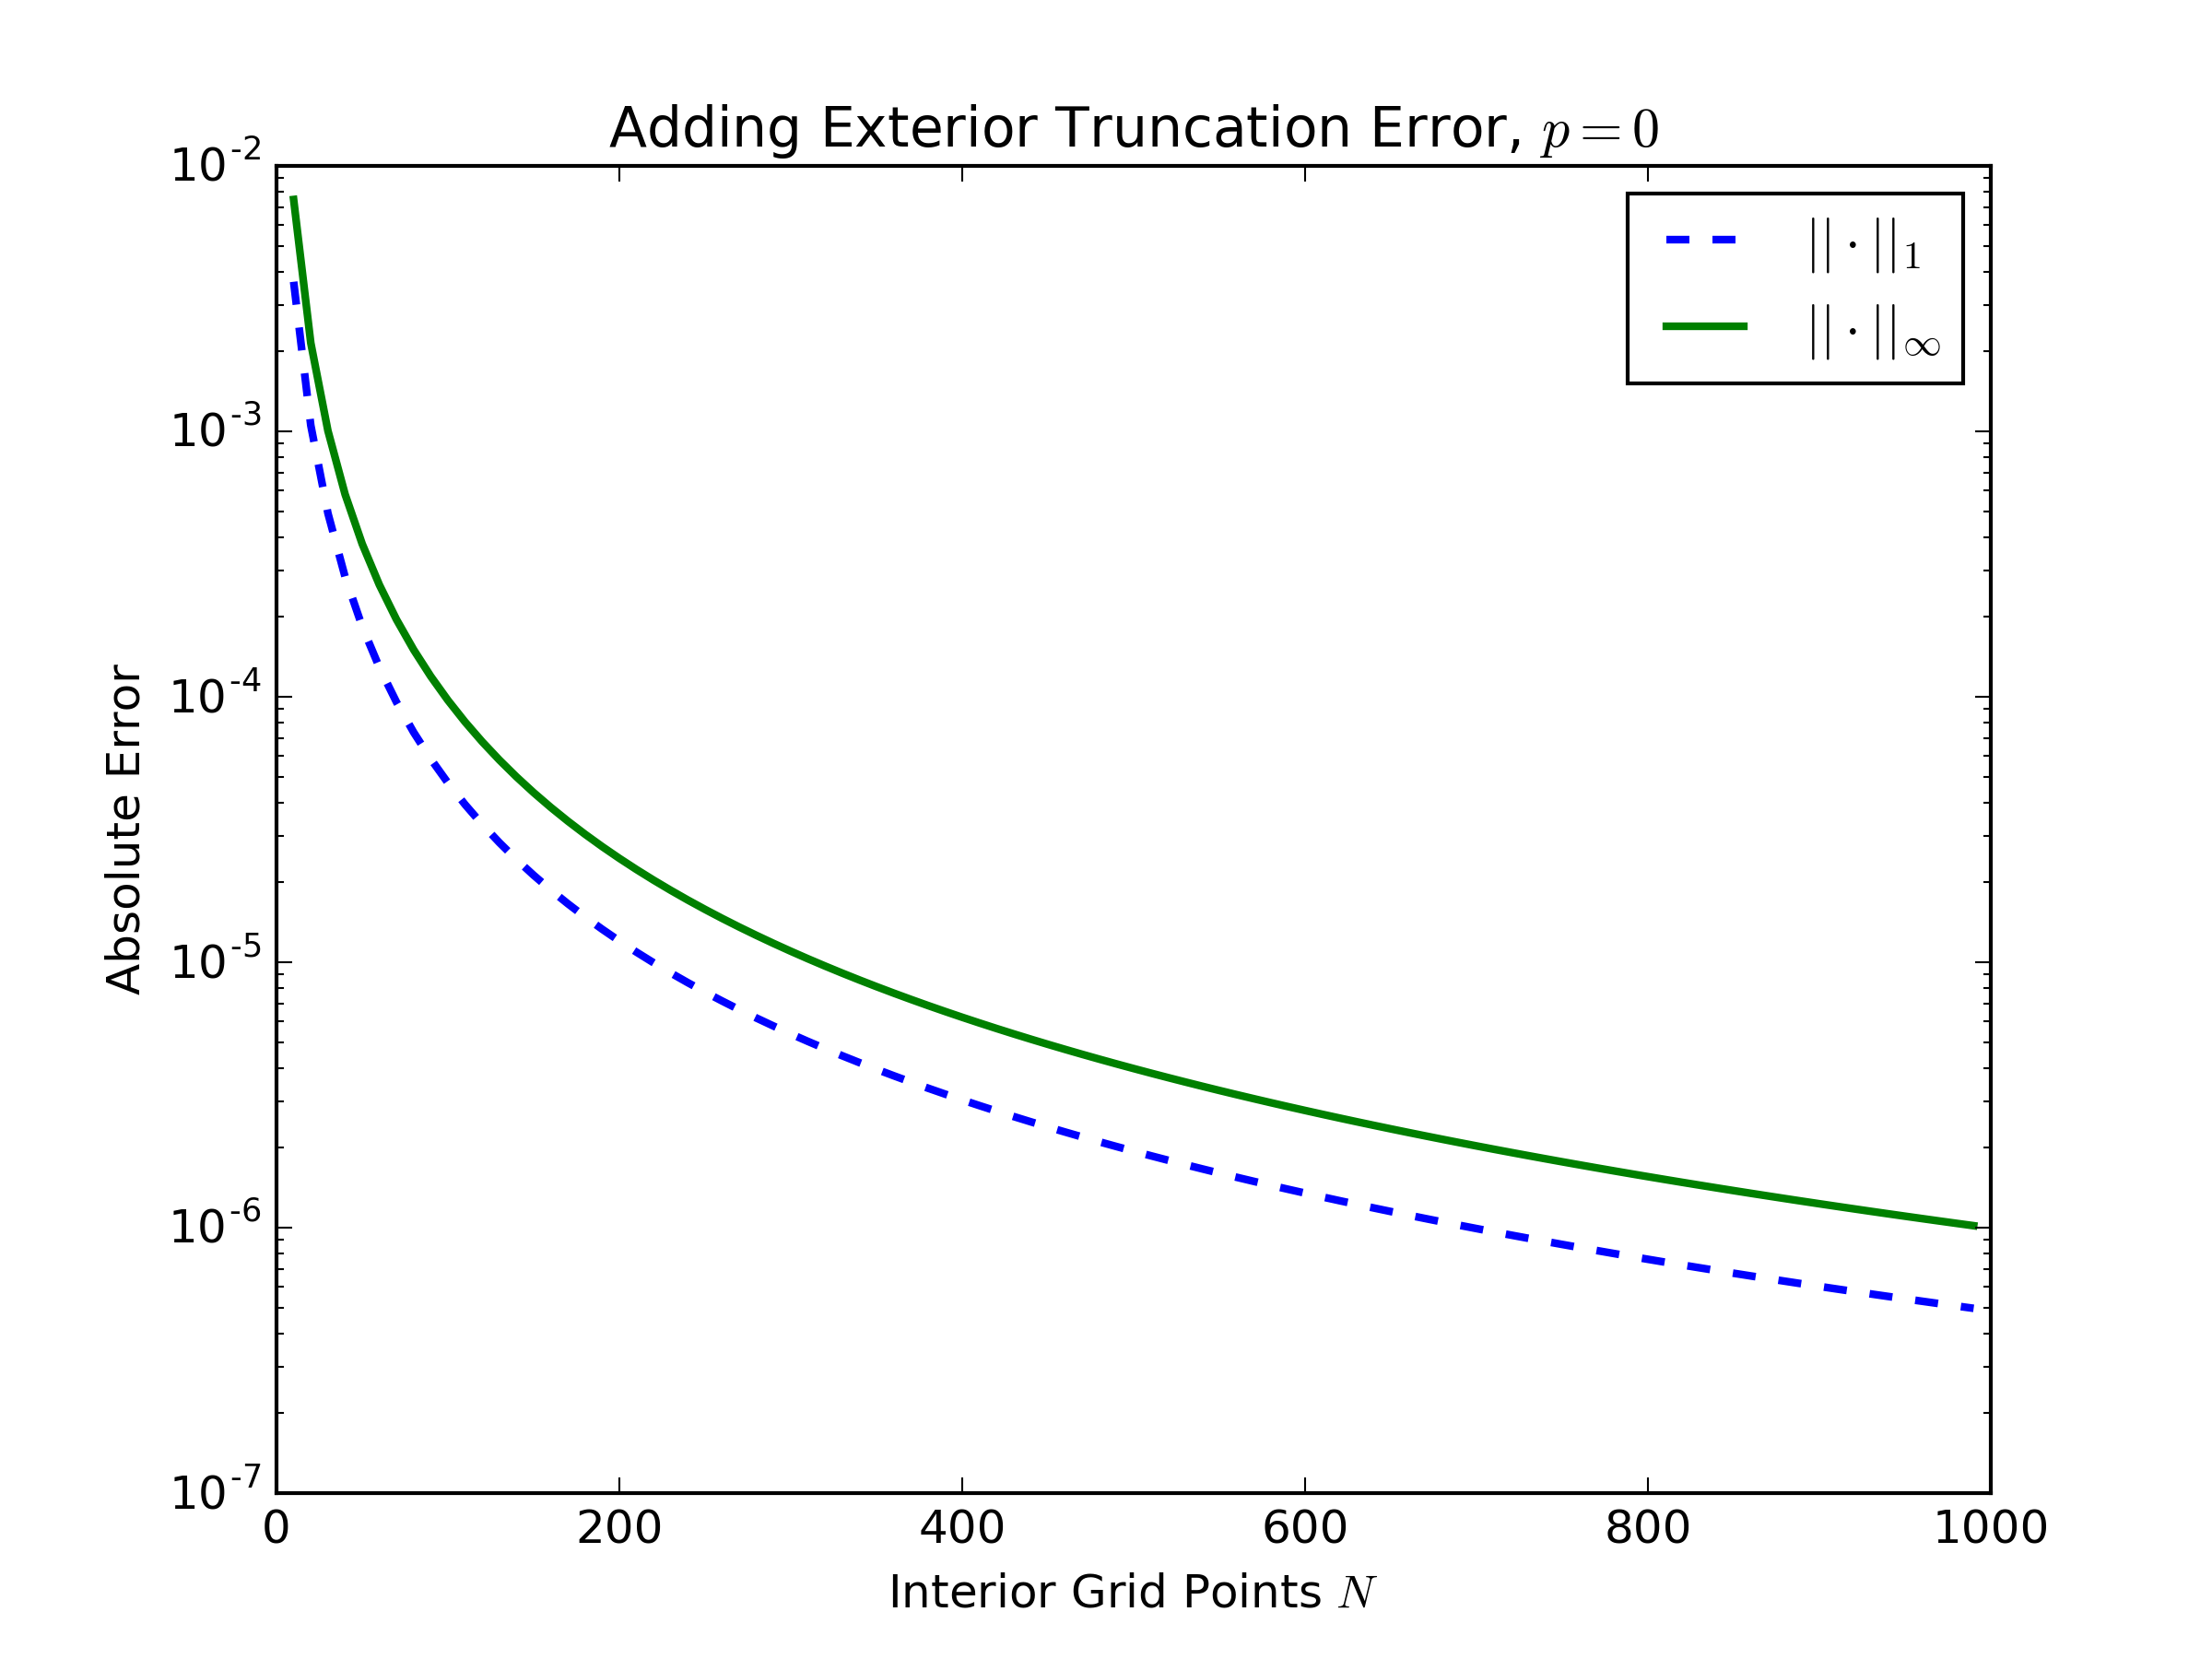
\includegraphics[width=\linewidth]{figure_2c1_ext_p=0.png}
                \vspace{4ex}
            \end{minipage} 
            \begin{minipage}[b]{0.5\linewidth}
                \centering
                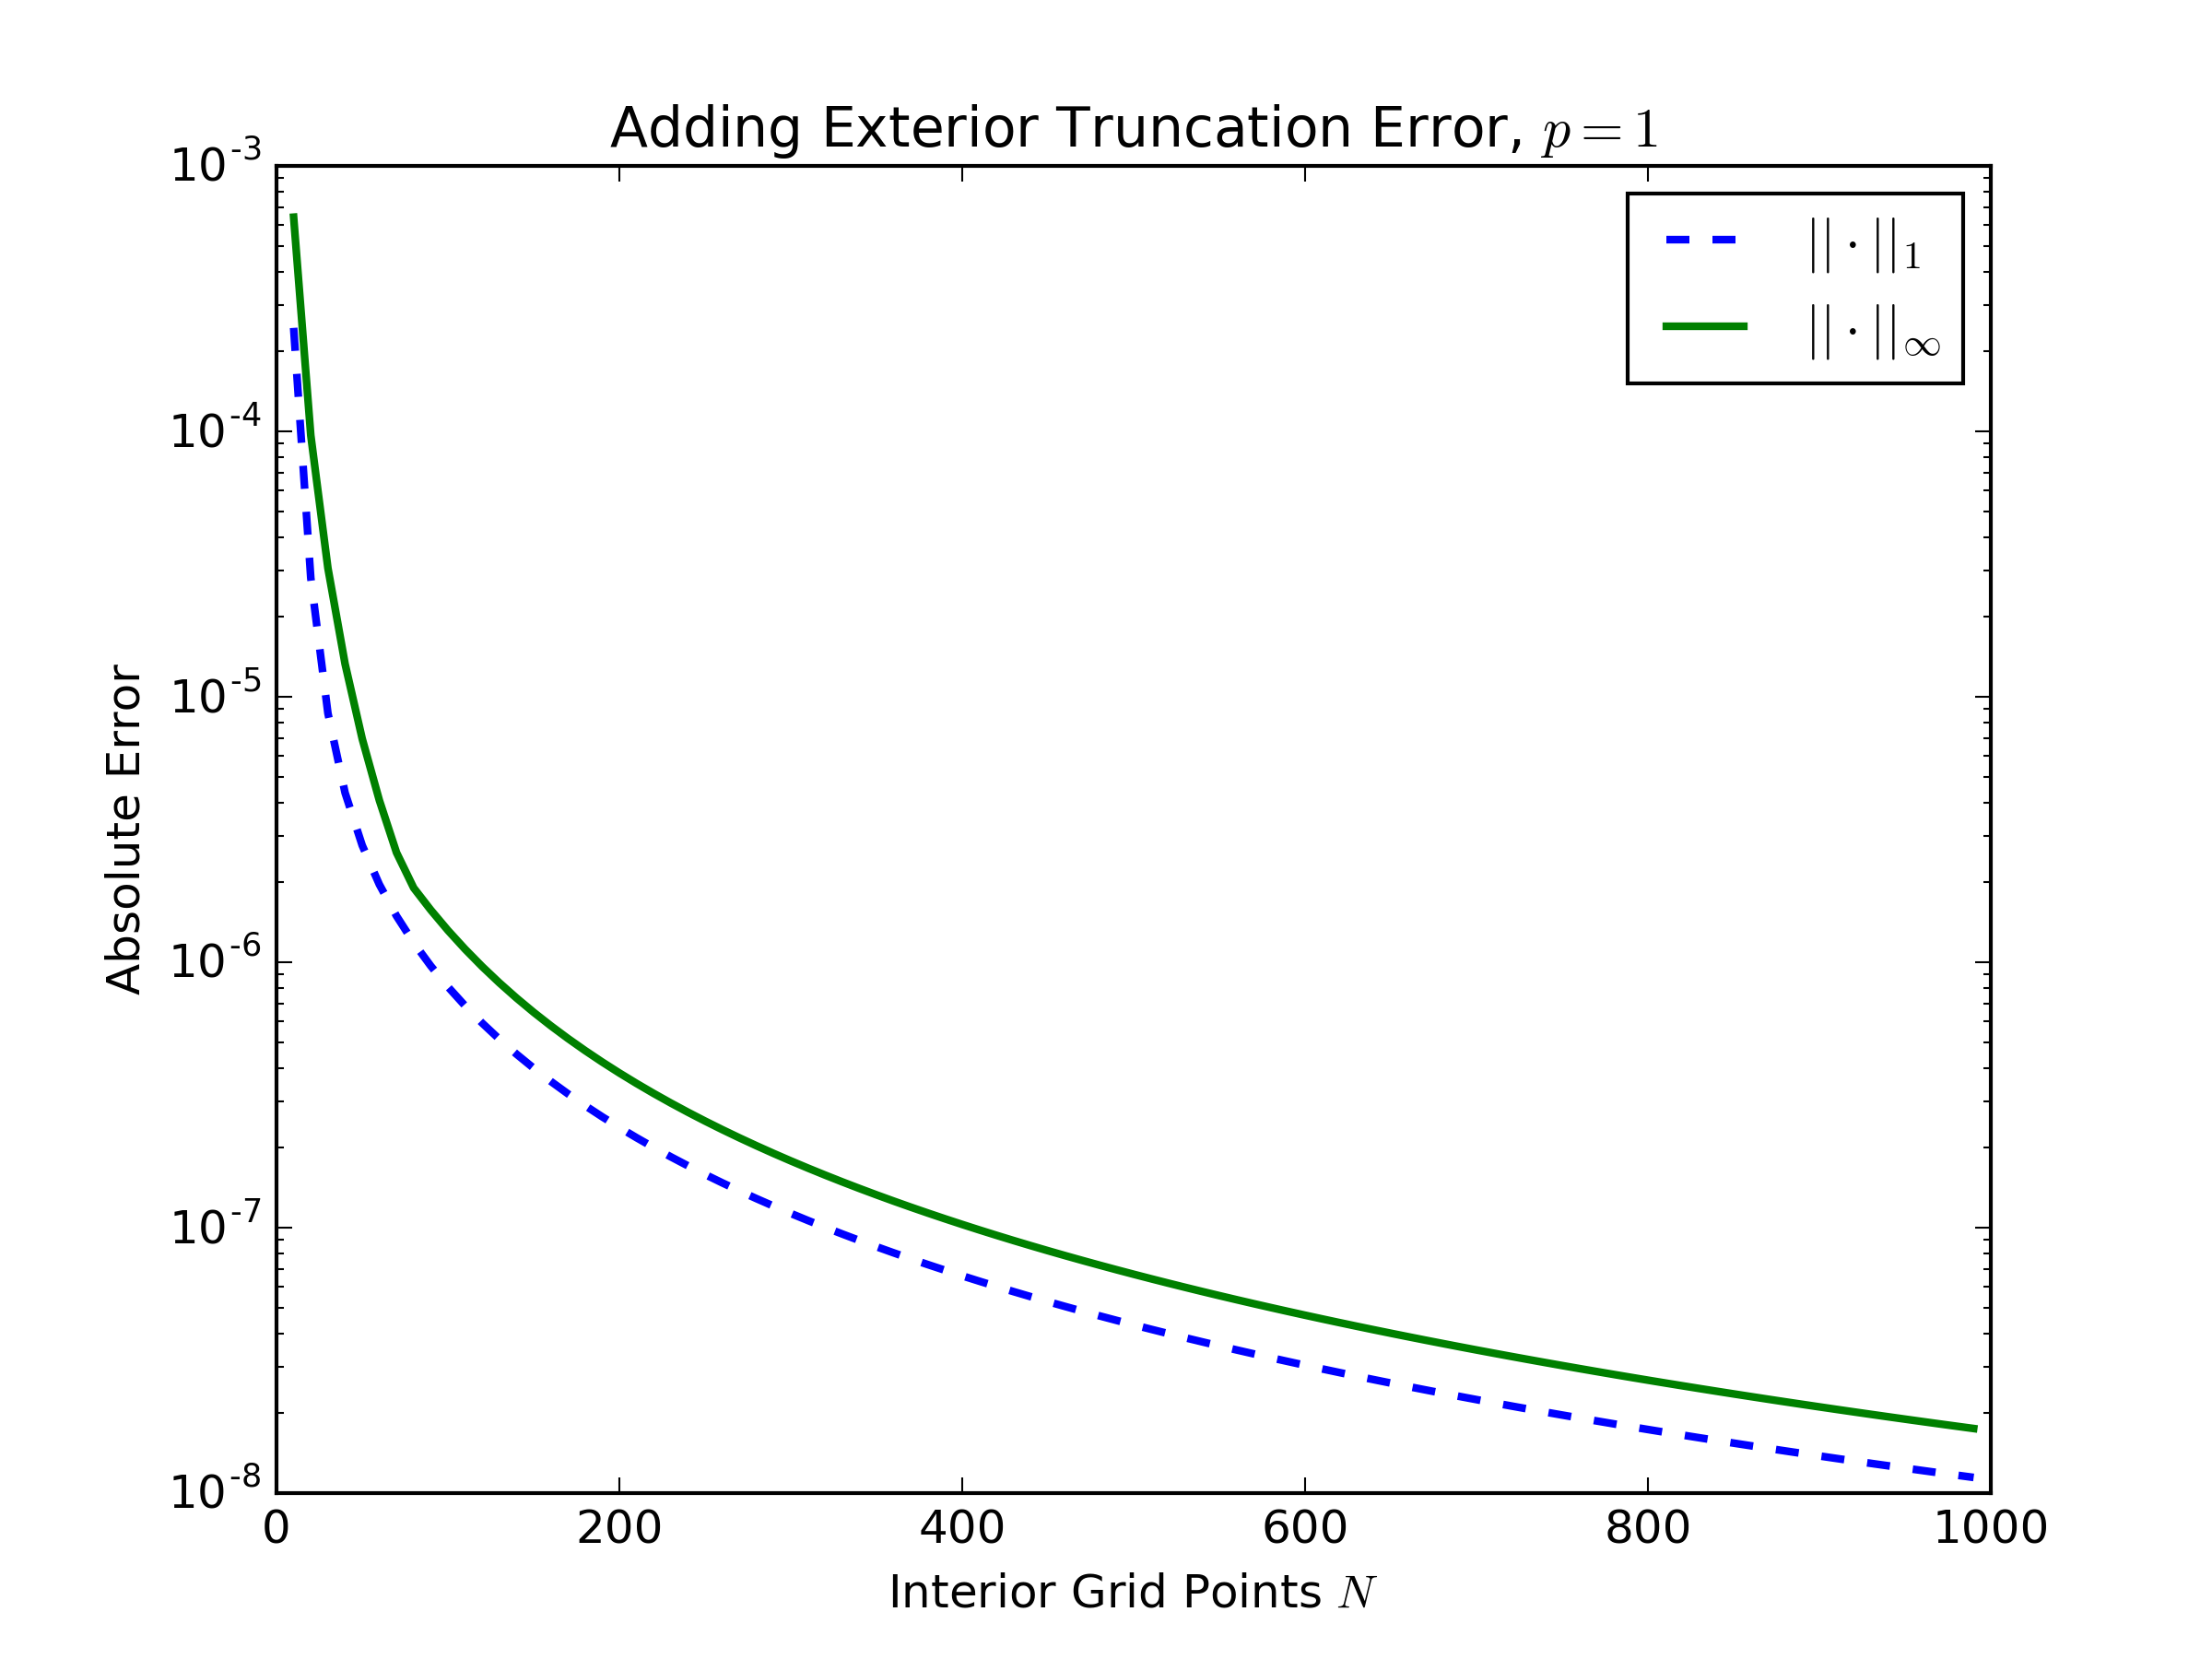
\includegraphics[width=\linewidth]{figure_2c1_ext_p=1.png} 
                \vspace{4ex}
            \end{minipage}%% 
            \begin{minipage}[b]{0.5\linewidth}
                \centering
                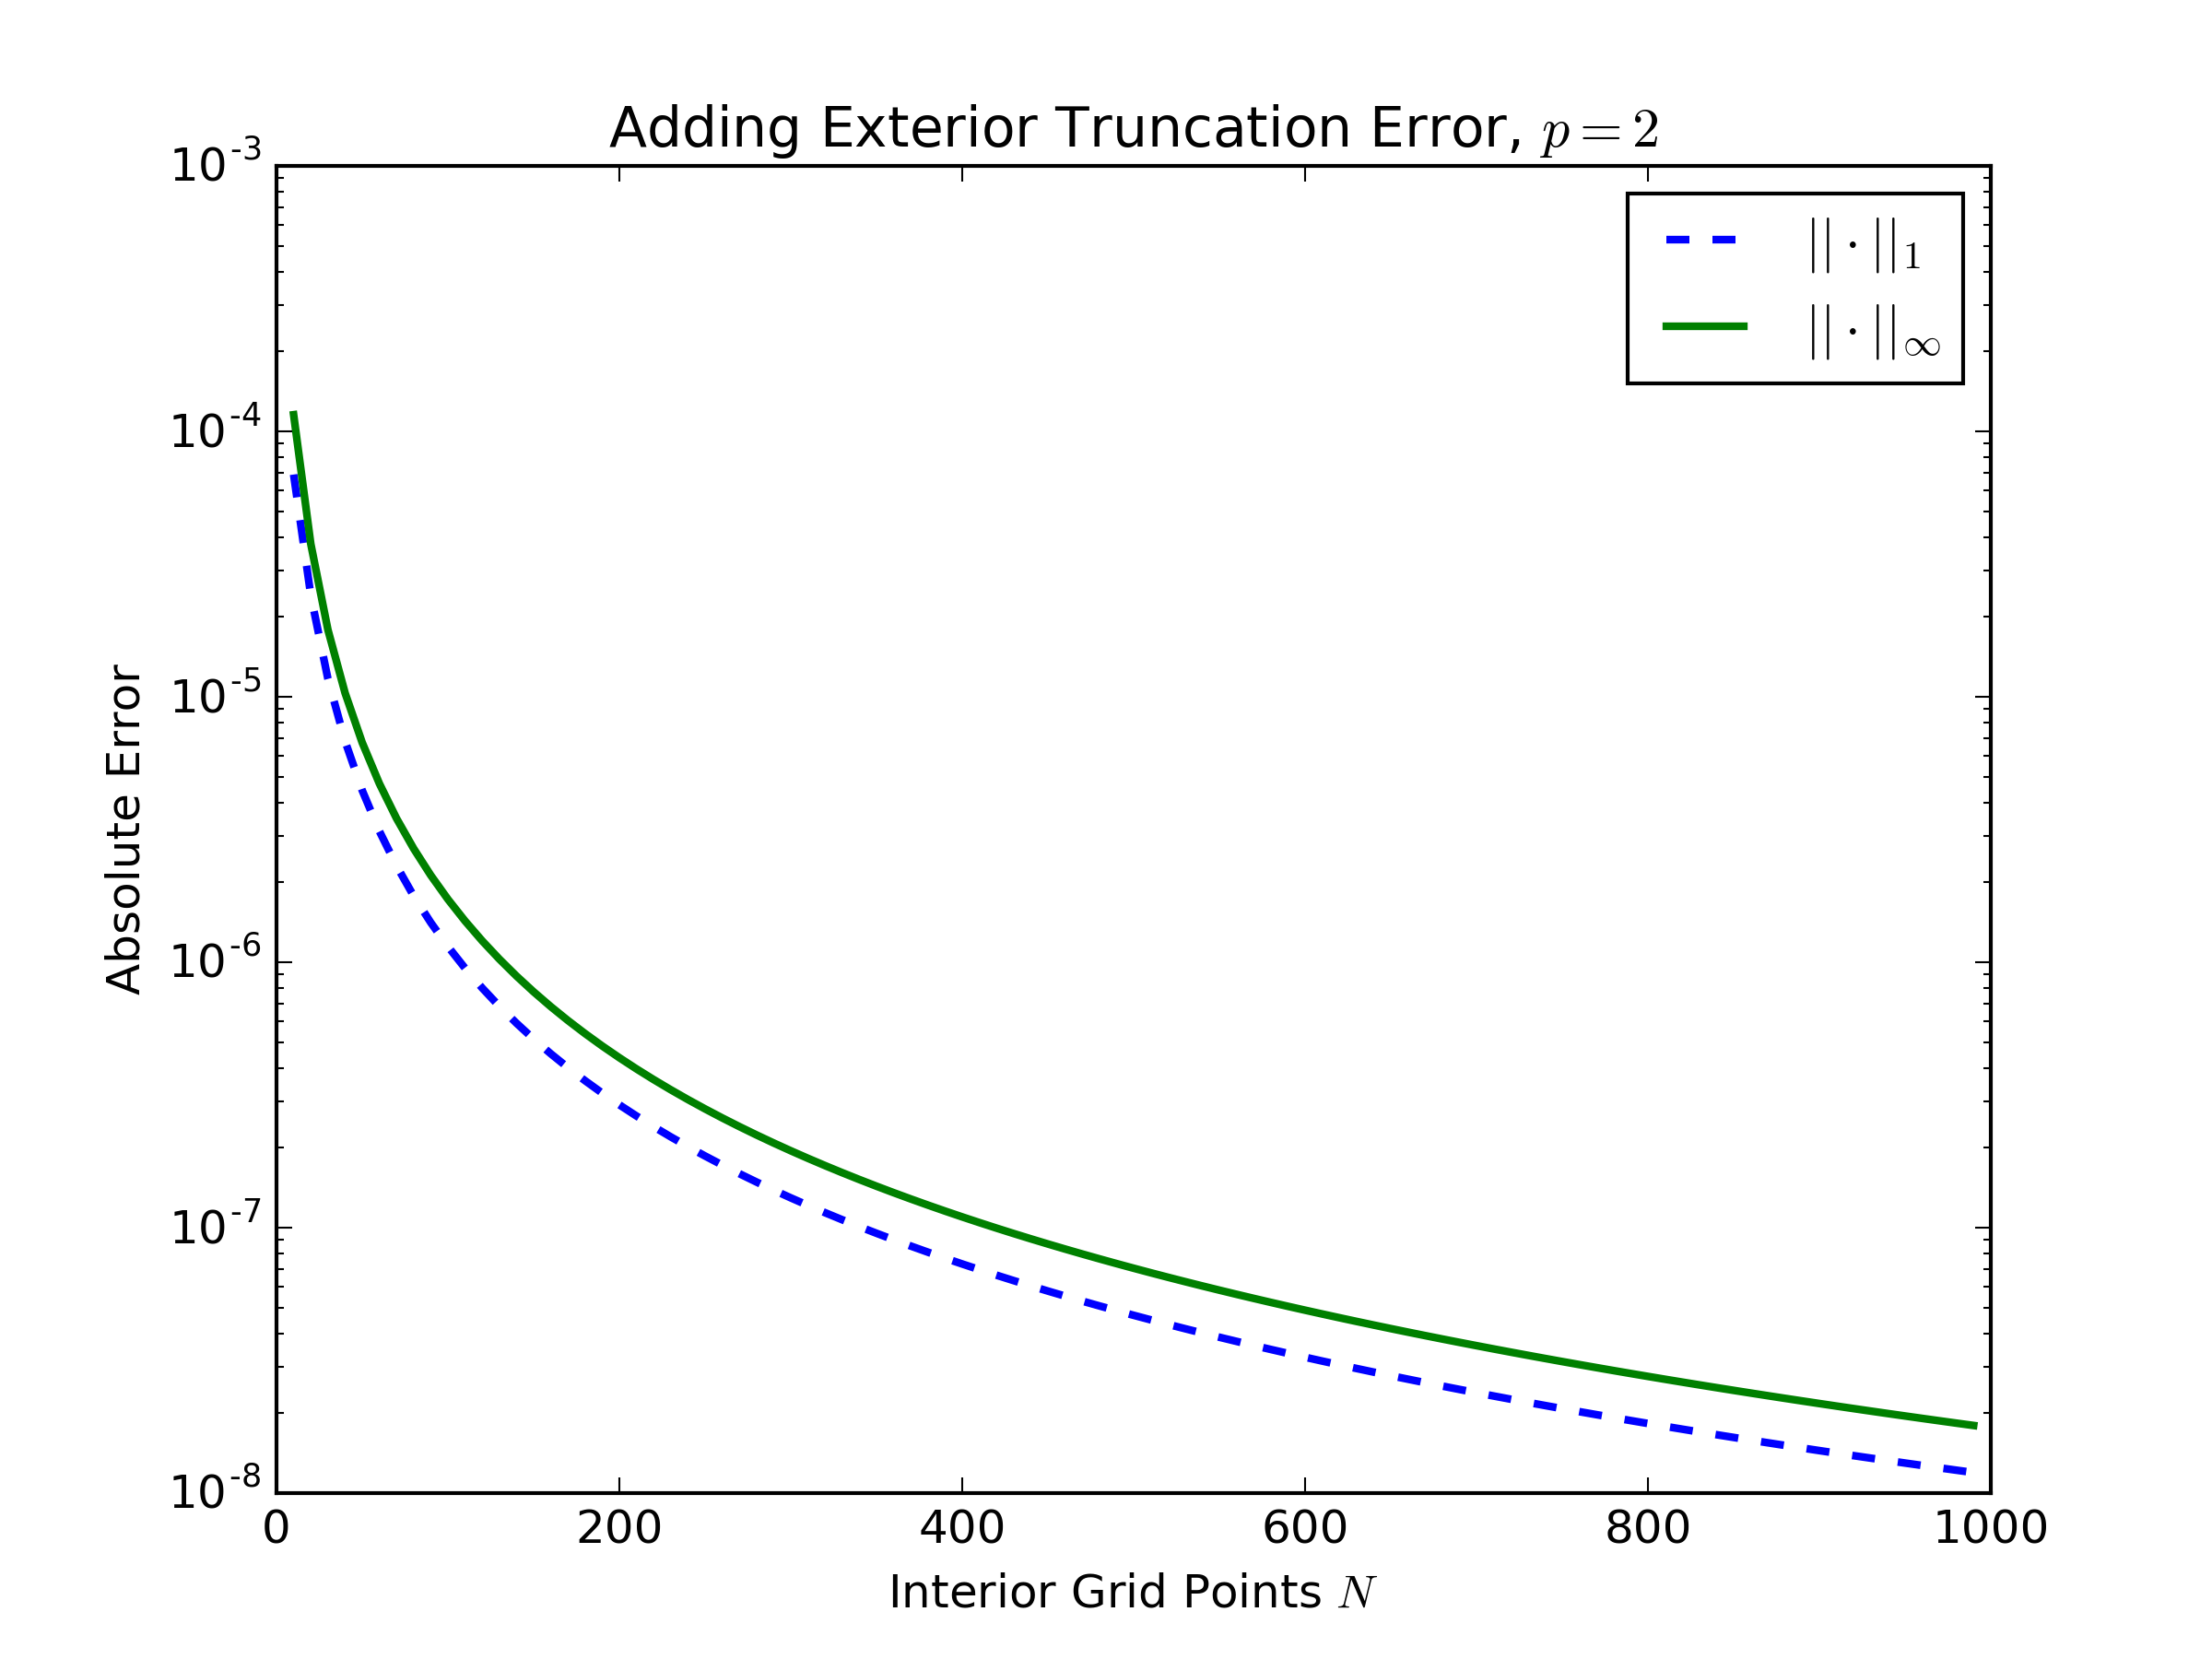
\includegraphics[width=\linewidth]{figure_2c1_ext_p=2.png}
                \vspace{4ex}
            \end{minipage} 
        \end{figure}
        \begin{figure}[ht!]
            \begin{minipage}[b]{0.5\linewidth}
                \centering
                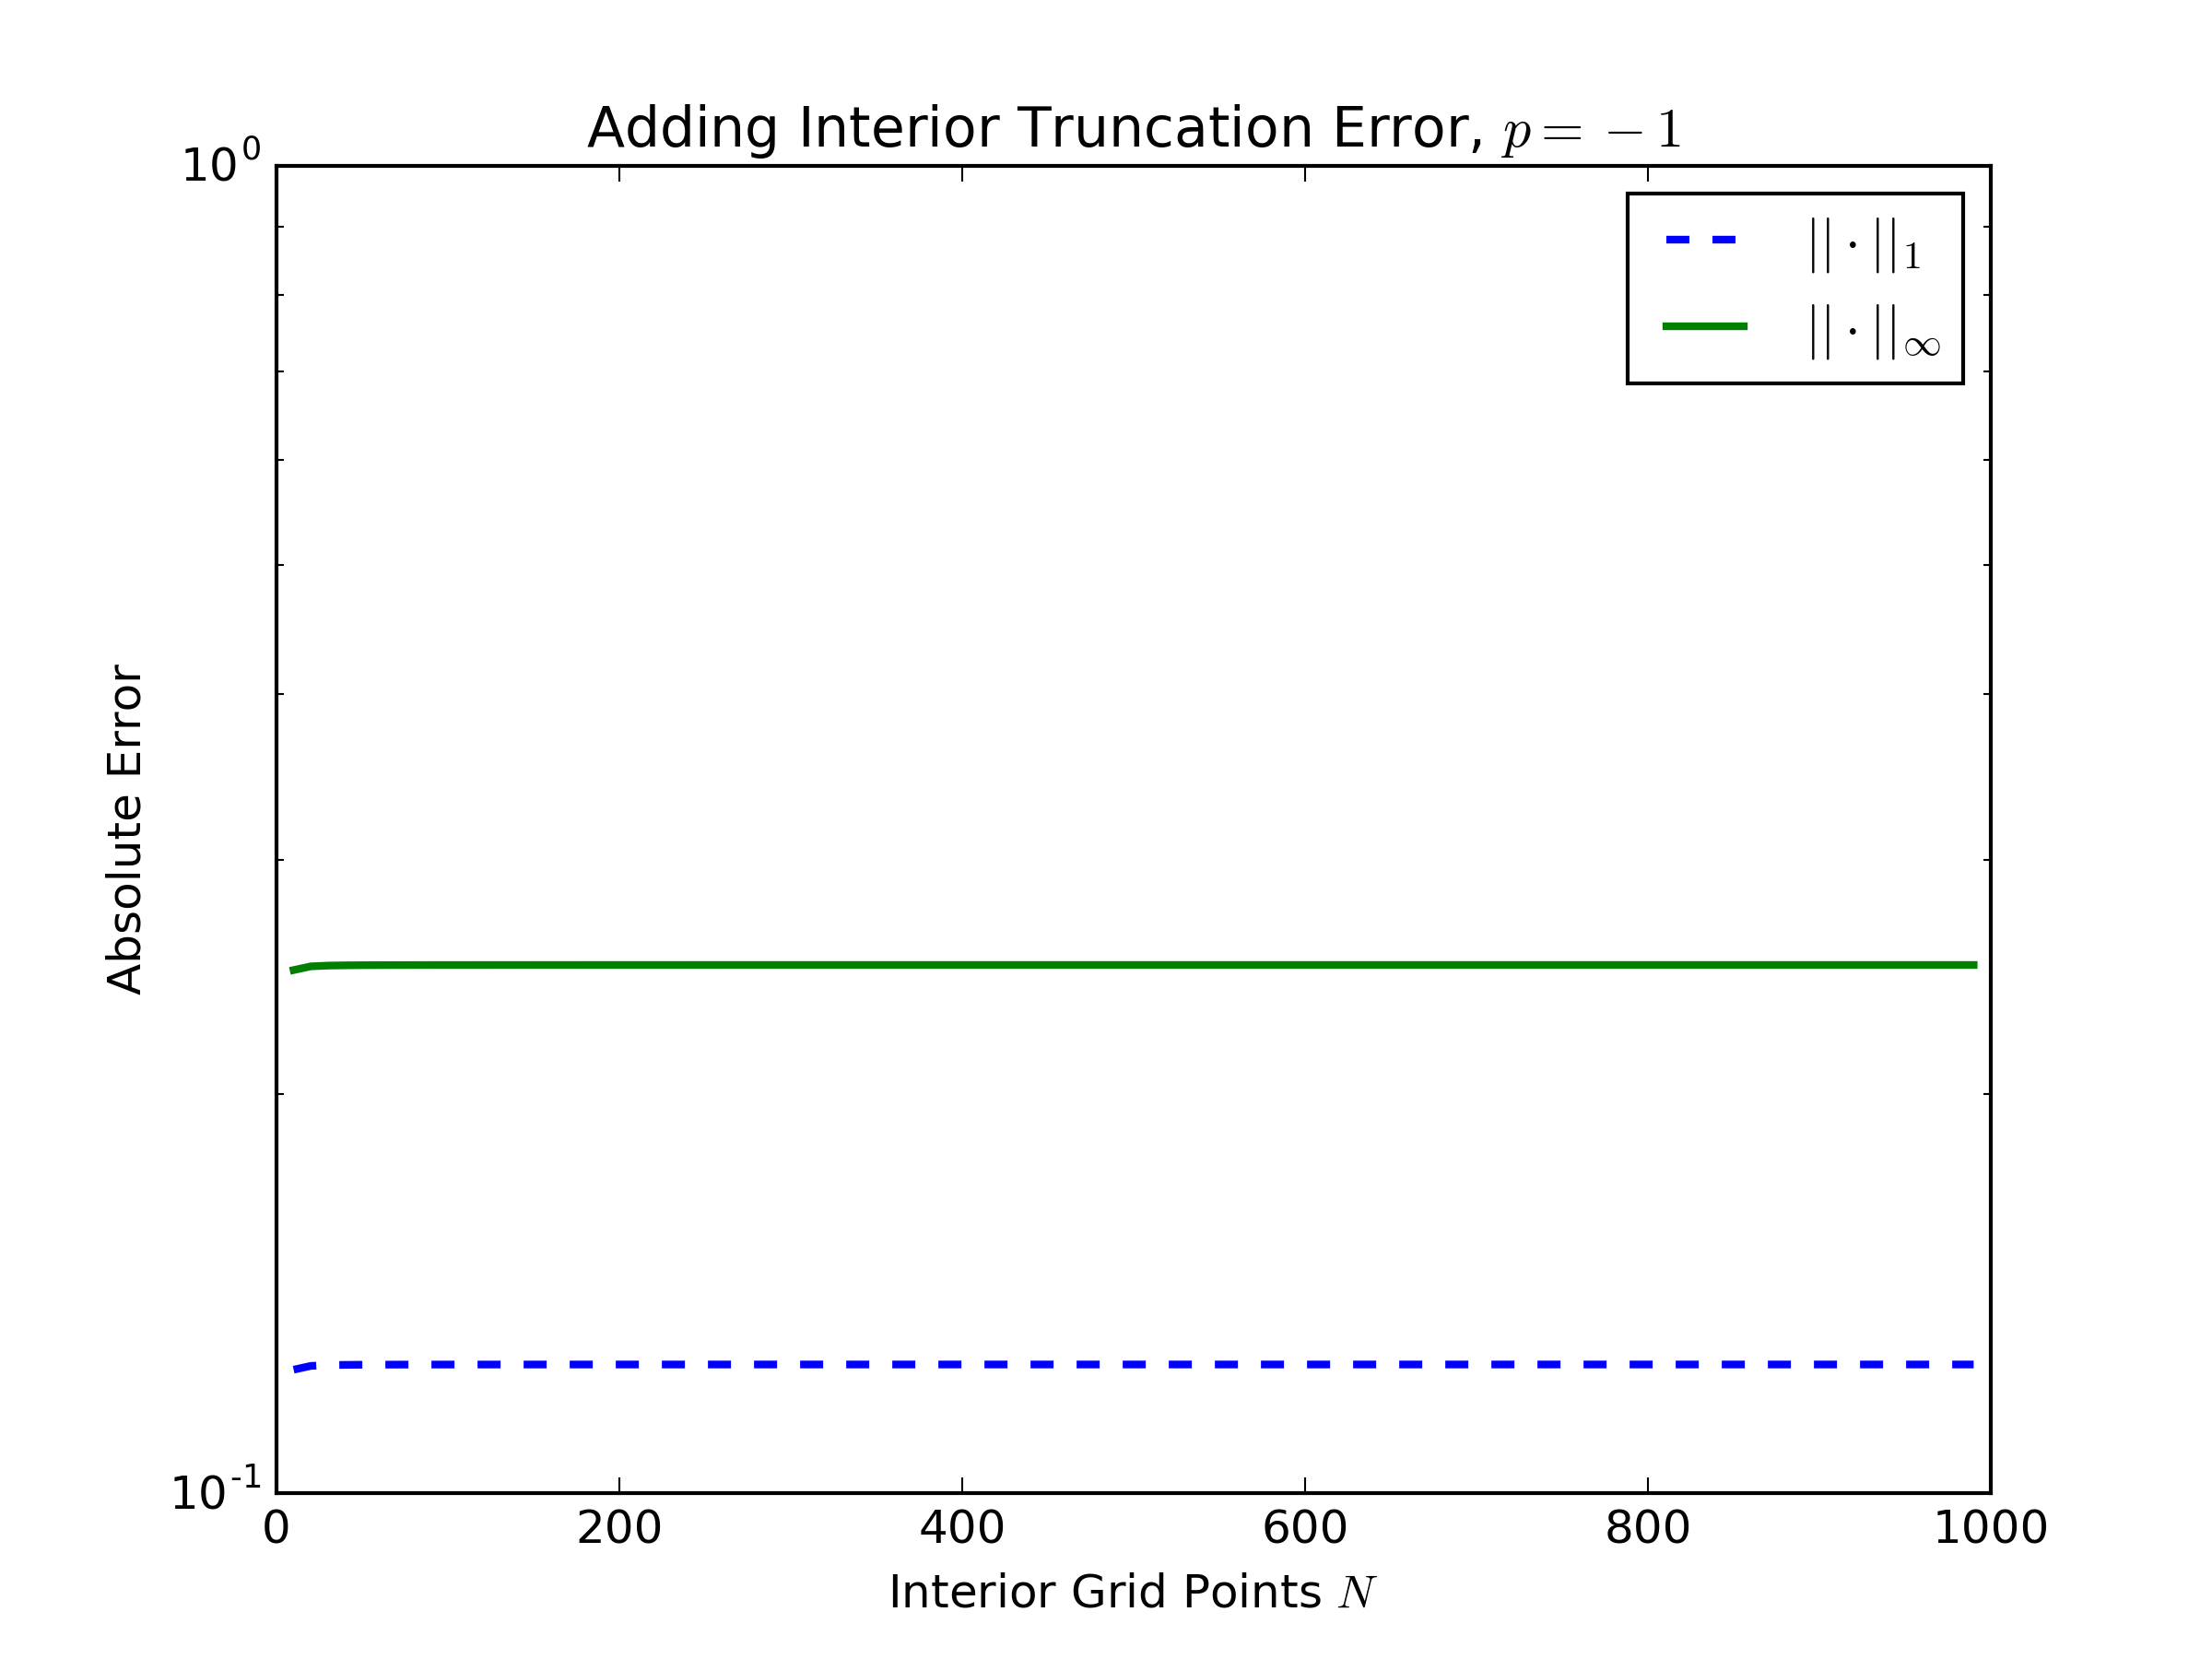
\includegraphics[width=\linewidth]{figure_2c1_int_p=-1.png}
                \vspace{4ex}
            \end{minipage}%%
            \begin{minipage}[b]{0.5\linewidth}
                \centering
                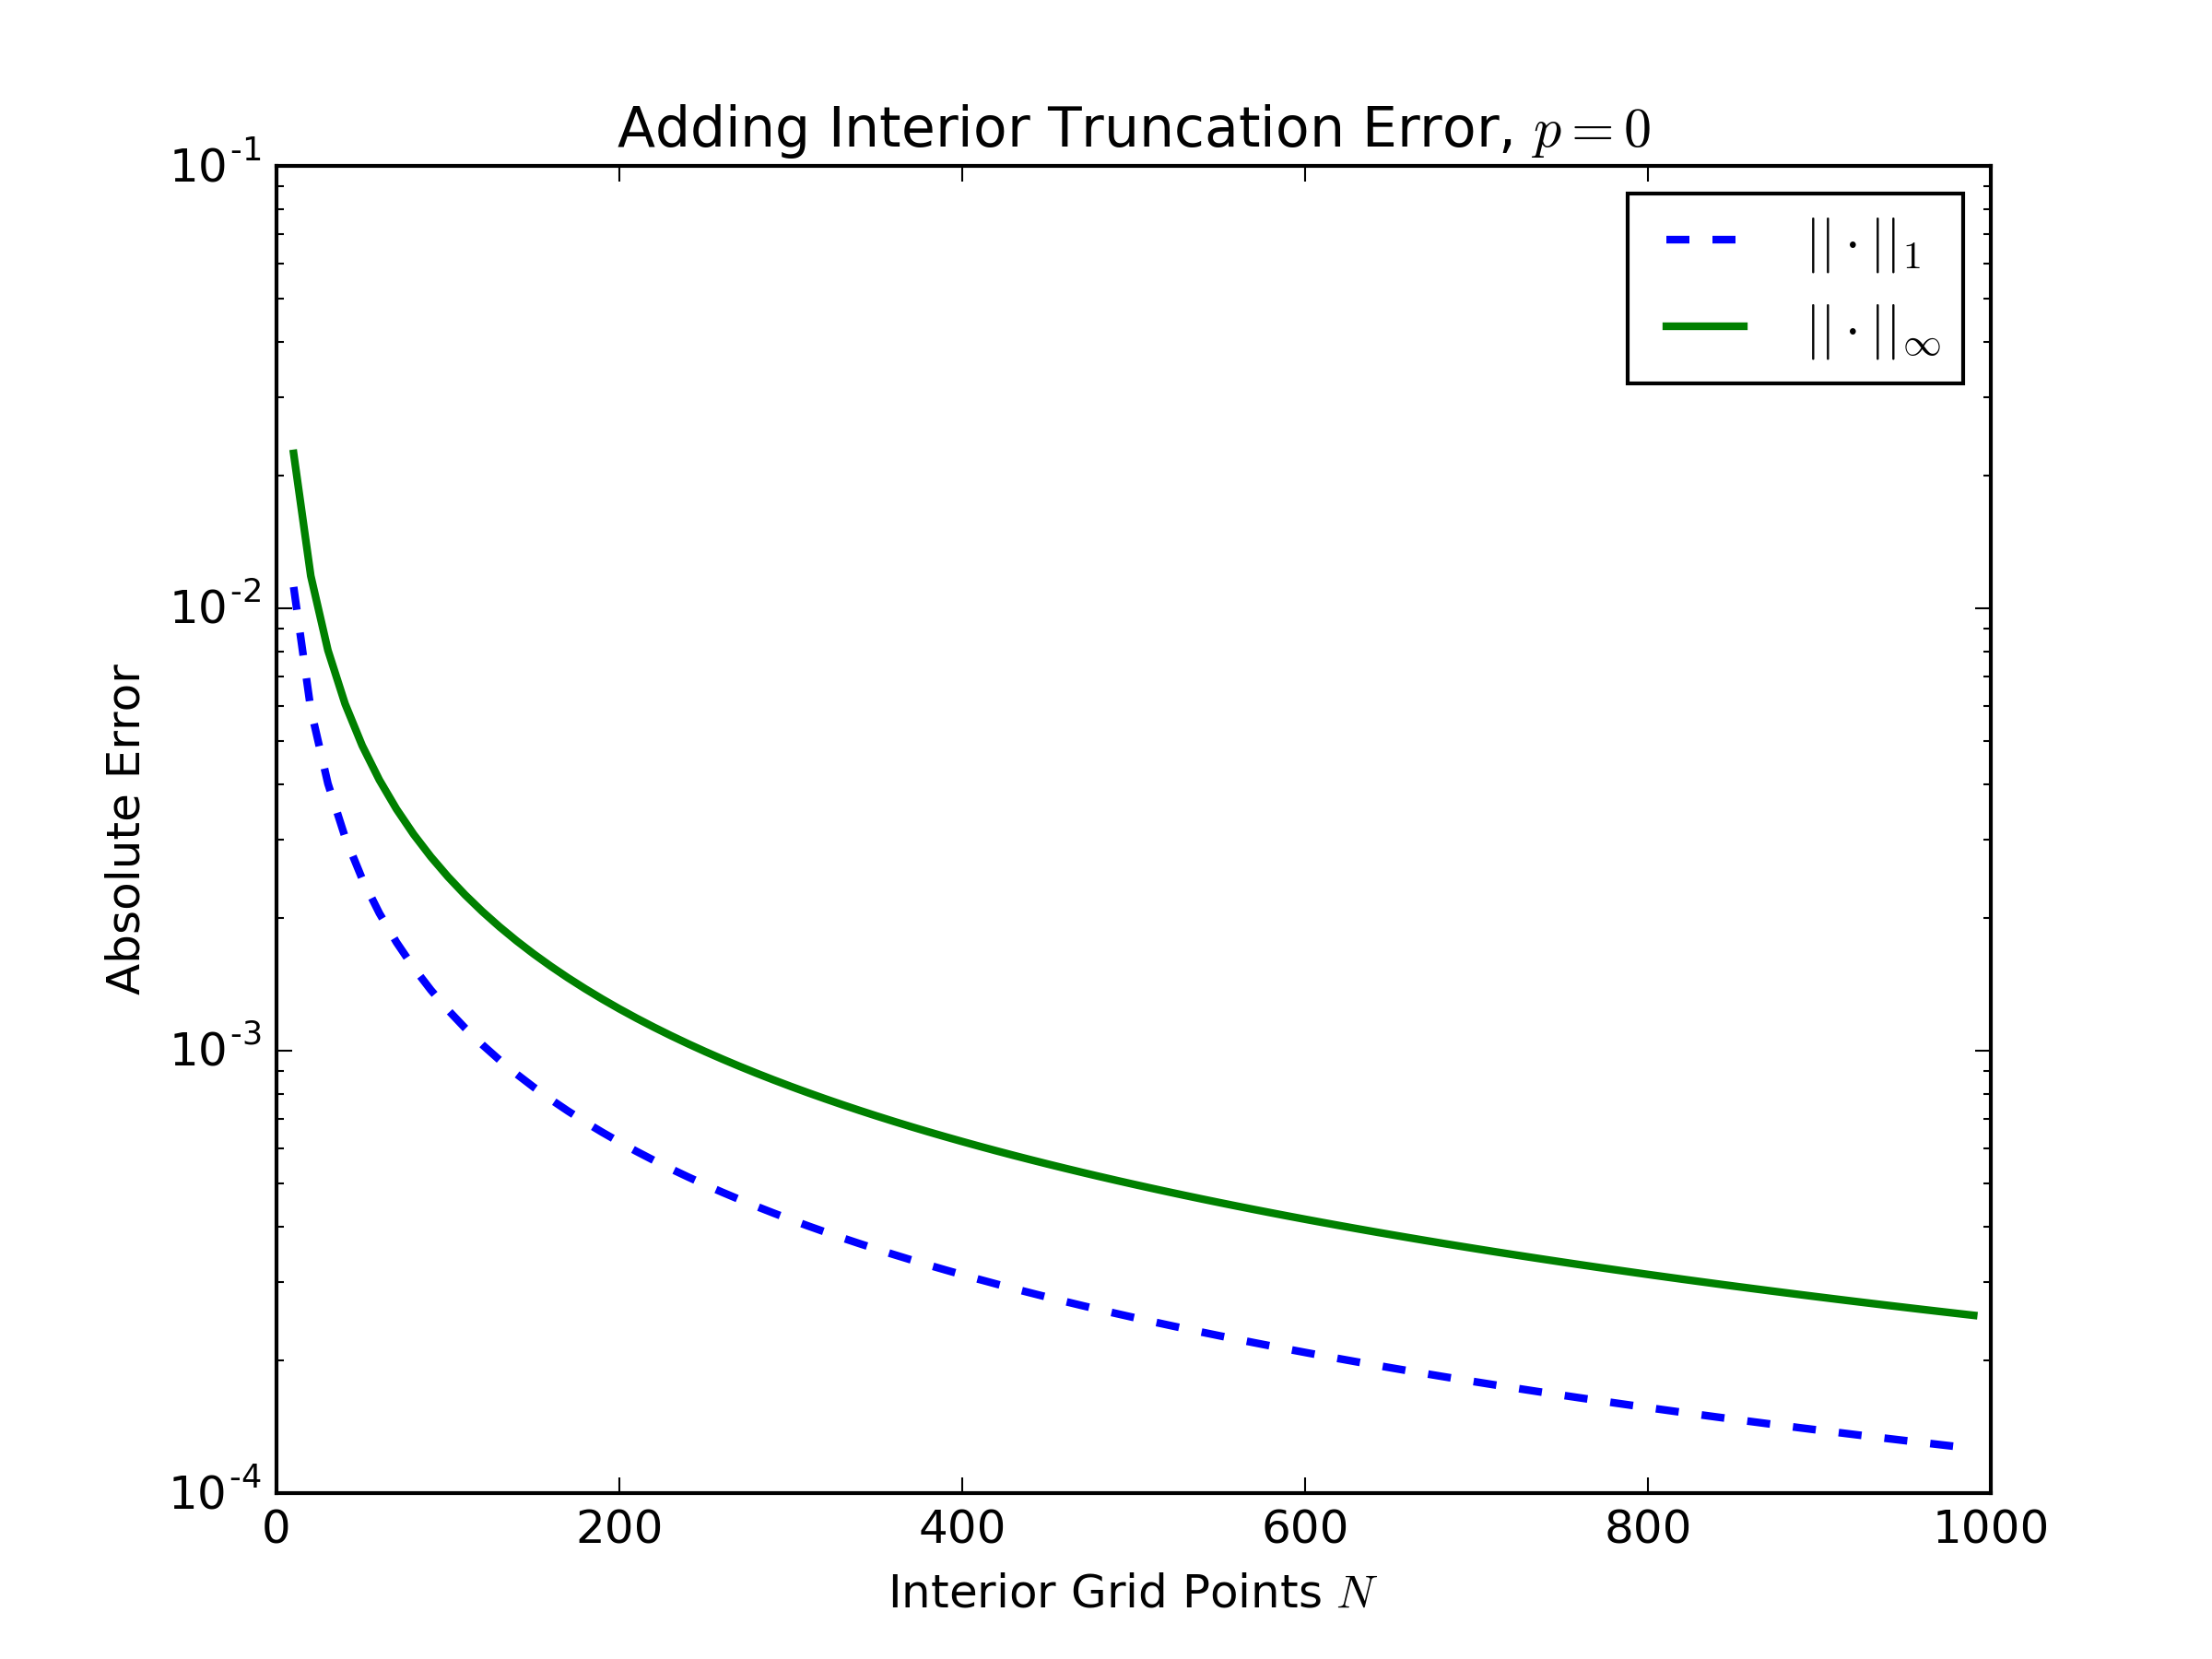
\includegraphics[width=\linewidth]{figure_2c1_int_p=0.png}
                \vspace{4ex}
            \end{minipage} 
            \begin{minipage}[b]{0.5\linewidth}
                \centering
                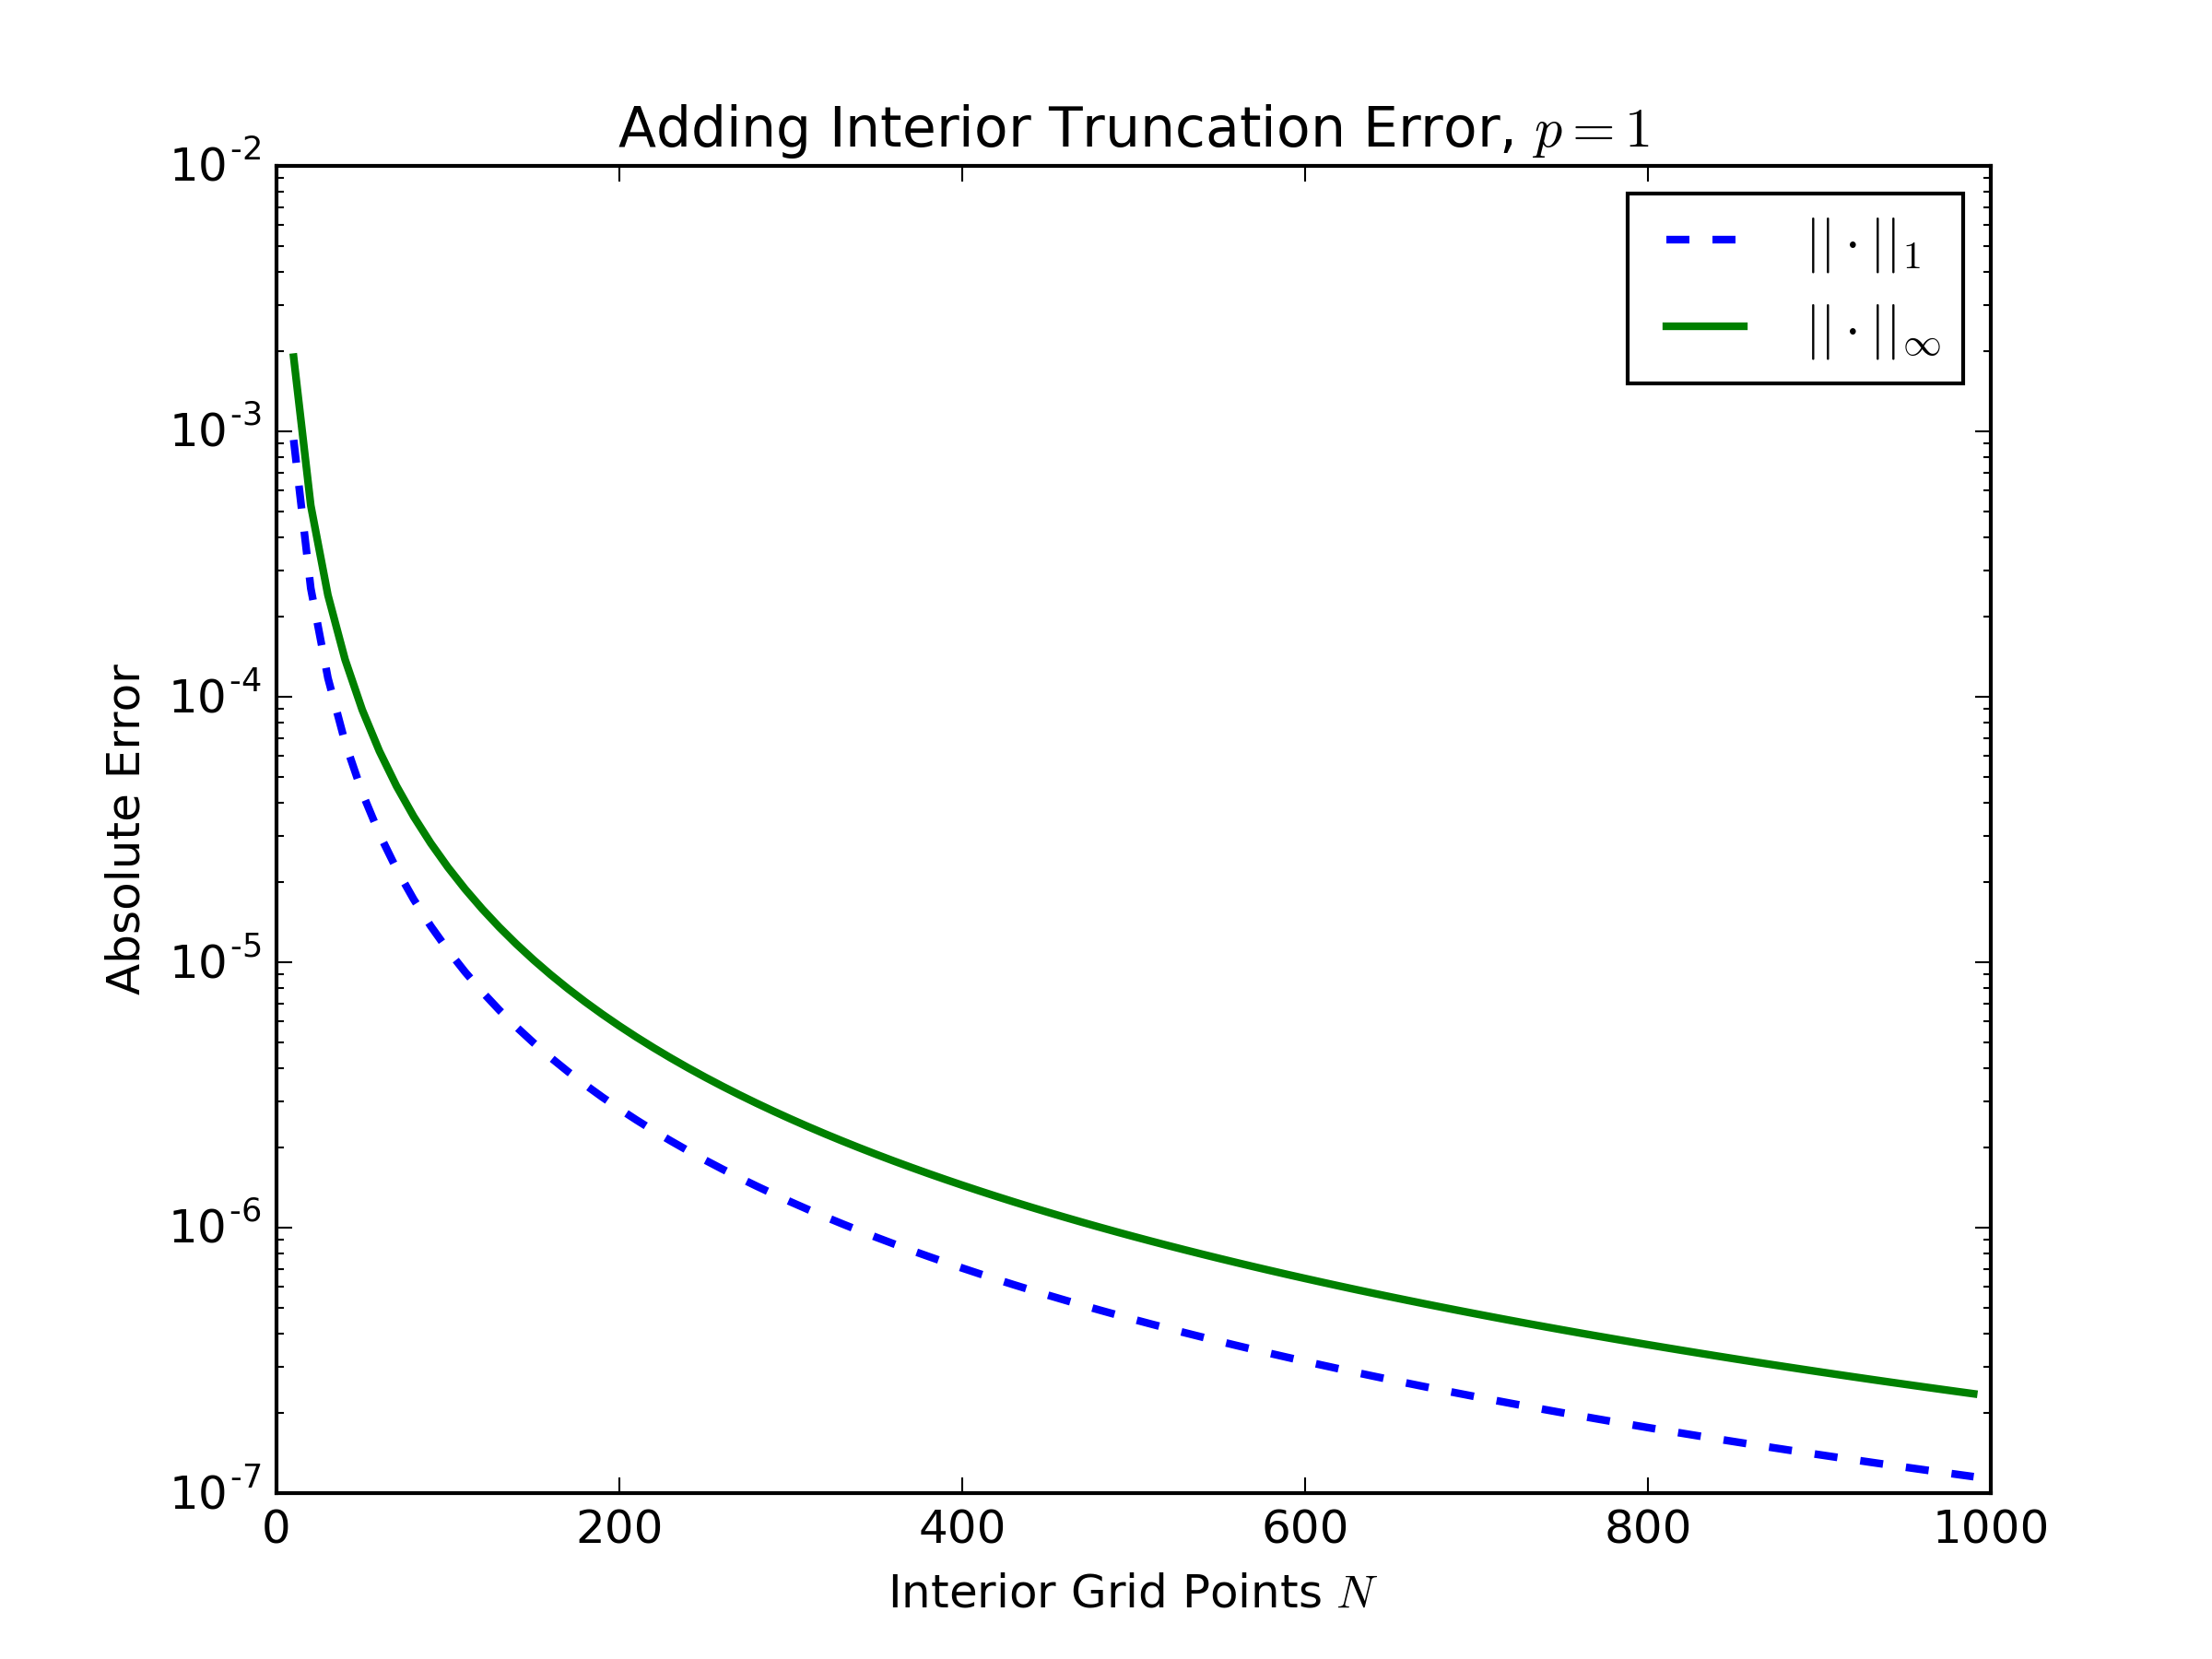
\includegraphics[width=\linewidth]{figure_2c1_int_p=1.png} 
                \vspace{4ex}
            \end{minipage}%% 
            \begin{minipage}[b]{0.5\linewidth}
                \centering
                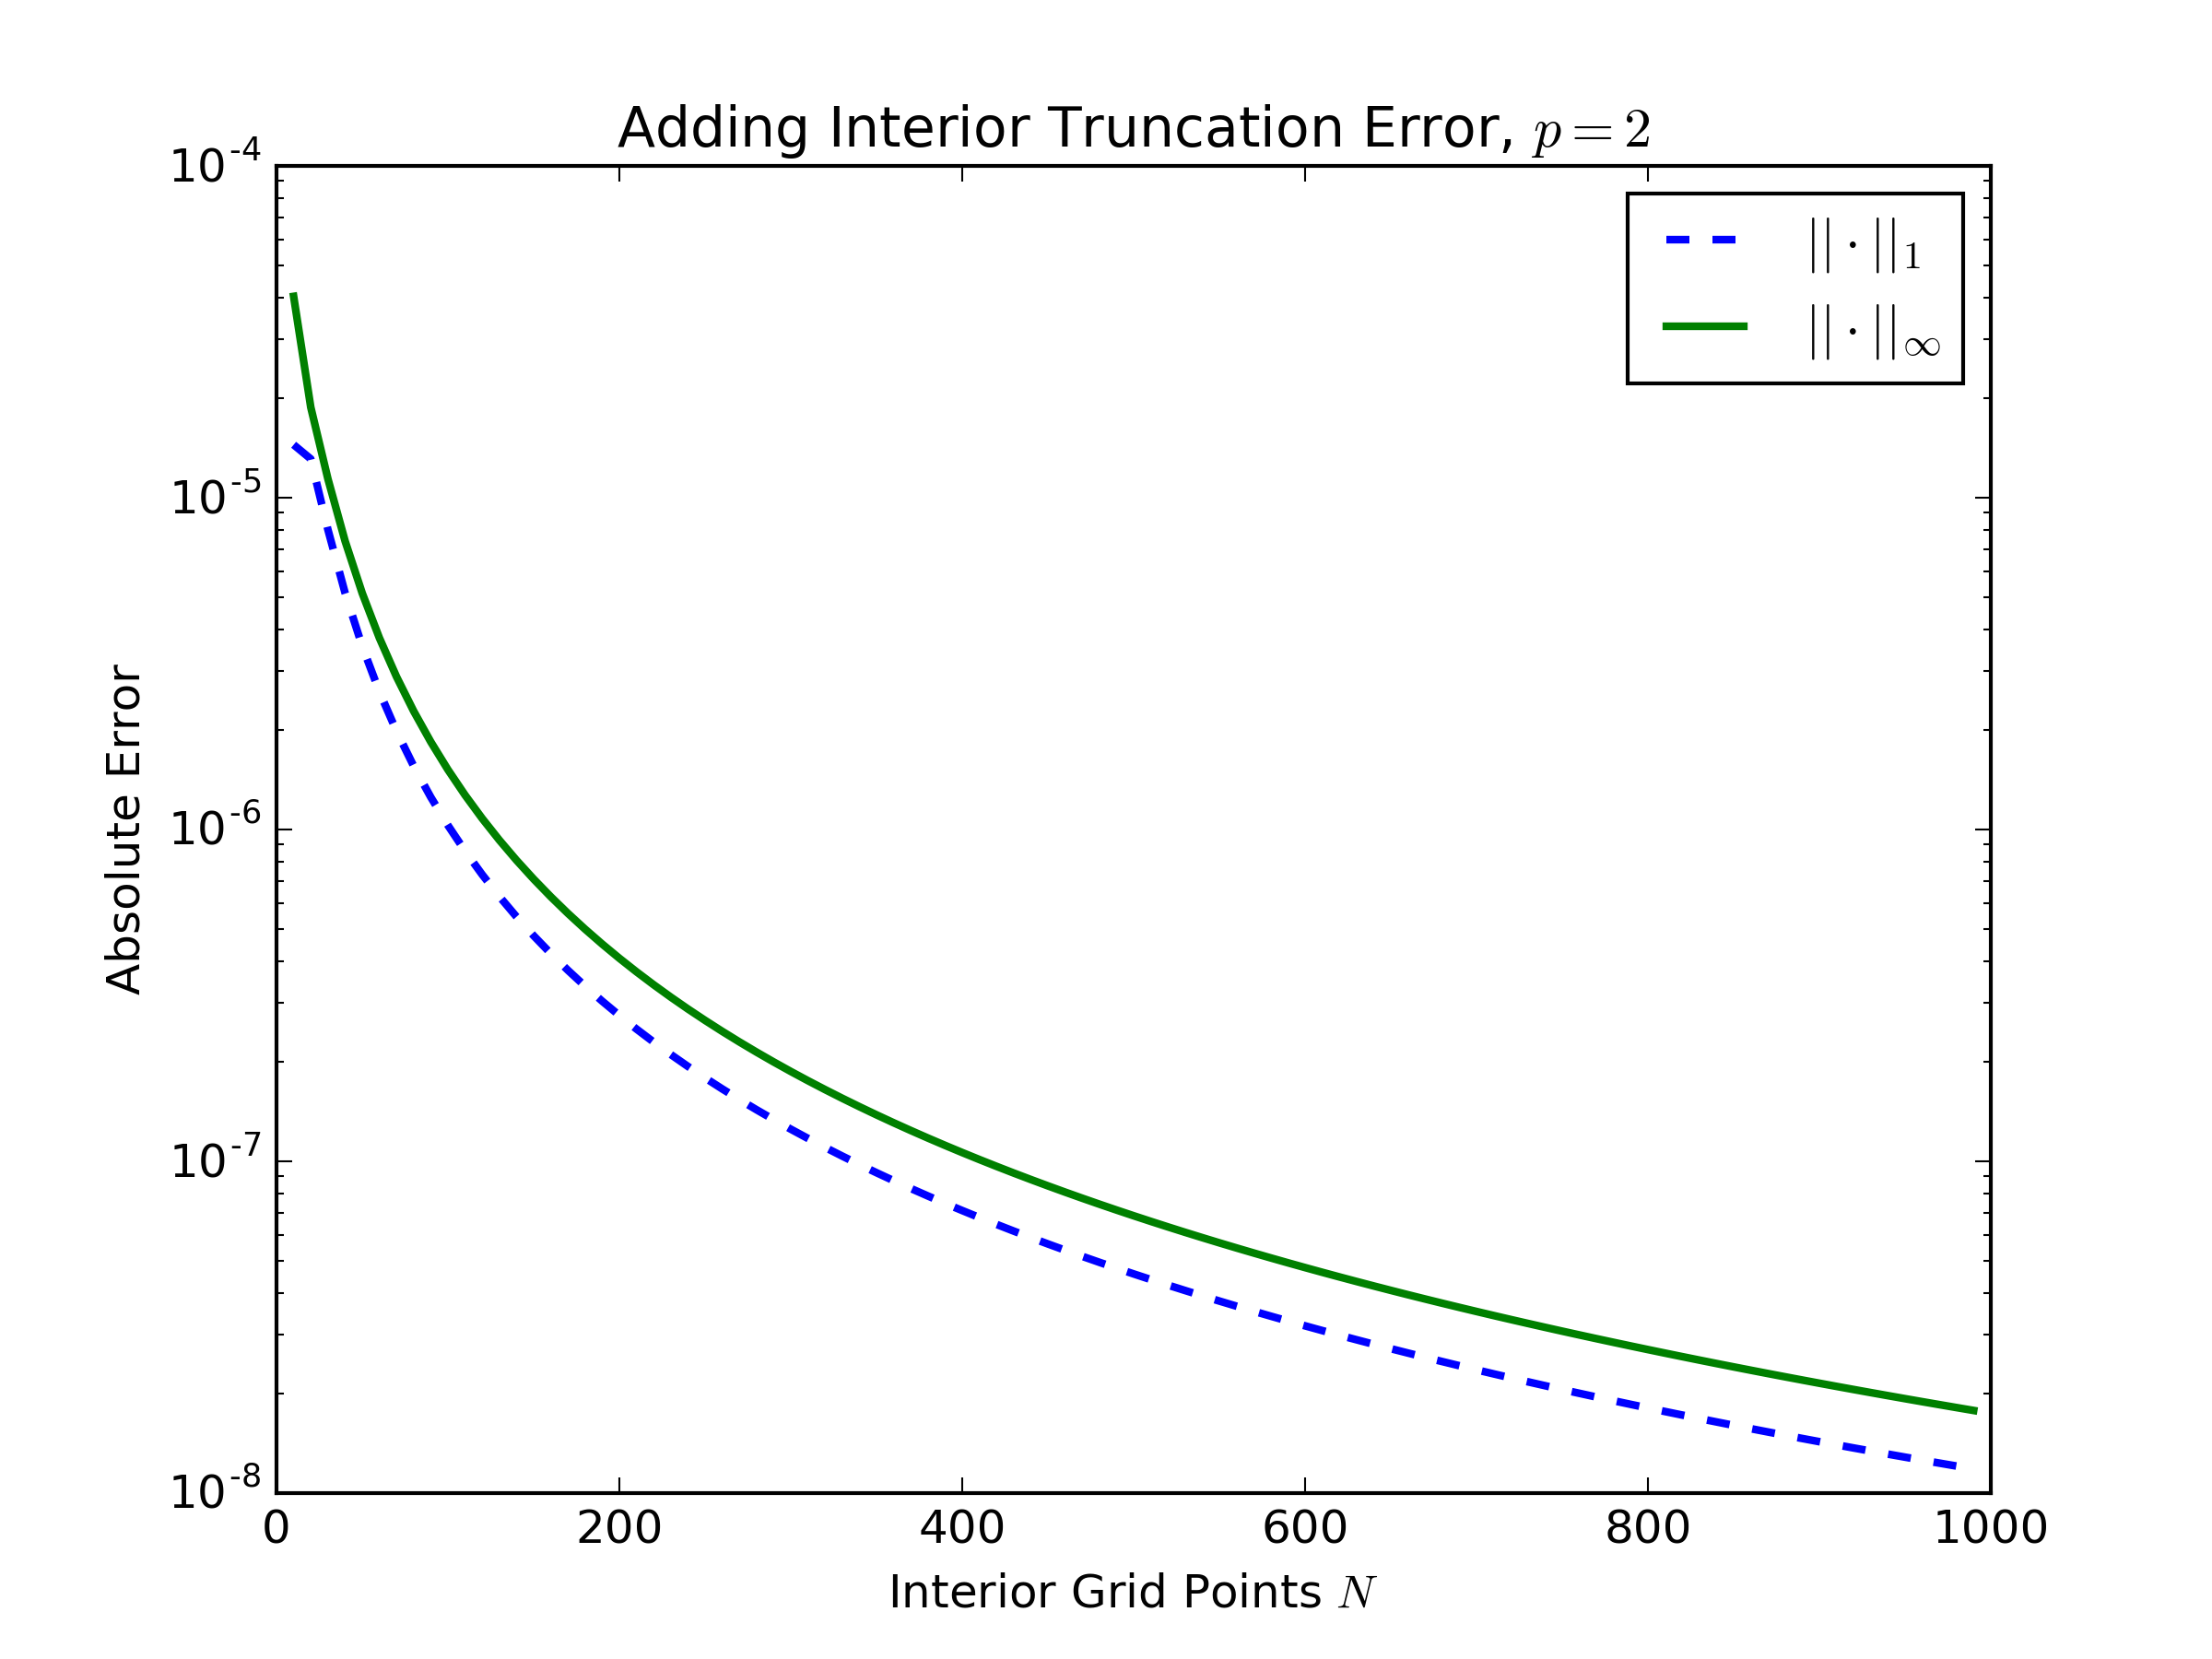
\includegraphics[width=\linewidth]{figure_2c1_int_p=2.png}
                \vspace{4ex}
            \end{minipage} 
        \end{figure}
        \FloatBarrier
        \begin{table*}
            \centering
            \caption{Exterior Point, $p=-1$}
            \begin{tabular}[ht!]{lllll}
                \hline
                    N &    one-norm &   one-norm ratios &    max norm &   max norm ratios \\
                \hline
                    2 & 0.10996     &          0        & 0.220591    &          0        \\
                    4 & 0.0795504   &          0.723447 & 0.159593    &          0.72348  \\
                    8 & 0.0492397   &          0.618975 & 0.09869     &          0.618384 \\
                   16 & 0.0276412   &          0.56136  & 0.0553516   &          0.560864 \\
                   32 & 0.0146816   &          0.53115  & 0.0293831   &          0.530845 \\
                   64 & 0.00757119  &          0.515692 & 0.0151477   &          0.515524 \\
                  128 & 0.00384522  &          0.507875 & 0.00769182  &          0.507787 \\
                  256 & 0.00193778  &          0.503945 & 0.00387591  &          0.5039   \\
                  512 & 0.000972714 &          0.501974 & 0.00194552  &          0.501952 \\
                 1024 & 0.000487318 &          0.500988 & 0.000974658 &          0.500976 \\
                \hline
            \end{tabular}
        \end{table*}
        \begin{table*}
            \centering
            \caption{Exterior Point, $p=0$}
            \begin{tabular}[ht!]{lllll}
                \hline
                    N &    one-norm &   one-norm ratios &    max norm &   max norm ratios \\
                \hline
                    2 & 0.0358862   &          0        & 0.0724429   &          0        \\
                    4 & 0.0155504   &          0.433326 & 0.0315933   &          0.436113 \\
                    8 & 0.00534396  &          0.343653 & 0.0108985   &          0.344961 \\
                   16 & 0.00158787  &          0.297133 & 0.00324499  &          0.297748 \\
                   32 & 0.000434455 &          0.273609 & 0.000888817 &          0.273904 \\
                   64 & 0.000113745 &          0.261811 & 0.000232829 &          0.261954 \\
                  128 & 2.9108e-05  &          0.255906 & 5.9599e-05  &          0.255977 \\
                  256 & 7.36296e-06 &          0.252953 & 1.50778e-05 &          0.252988 \\
                  512 & 1.85161e-06 &          0.251477 & 3.79199e-06 &          0.251494 \\
                 1024 & 4.6427e-07  &          0.250738 & 9.5083e-07  &          0.250747 \\
                \hline
            \end{tabular}
        \end{table*}
        \begin{table*}
            \centering
            \caption{Exterior Point, $p=1$}
            \begin{tabular}[ht!]{lllll}
                \hline
                    N &    one-norm &   one-norm ratios &    max norm &   max norm ratios \\
                \hline
                    2 & 0.0111949   &          0        & 0.0230602   &          0        \\
                    4 & 0.00275045  &          0.245688 & 0.0059933   &          0.259898 \\
                    8 & 0.000466653 &          0.169664 & 0.00114386  &          0.190856 \\
                   16 & 5.67118e-05 &          0.121529 & 0.000179896 &          0.157271 \\
                   32 & 7.34304e-06 &          0.12948  & 2.53532e-05 &          0.140933 \\
                   64 & 1.74856e-06 &          0.238125 & 3.3697e-06  &          0.13291  \\
                  128 & 5.26978e-07 &          0.301378 & 8.5965e-07  &          0.255112 \\
                  256 & 1.5185e-07  &          0.288152 & 2.41082e-07 &          0.280442 \\
                  512 & 4.11298e-08 &          0.270858 & 6.37409e-08 &          0.264395 \\
                 1024 & 1.07229e-08 &          0.260708 & 1.6382e-08  &          0.257009 \\
                \hline
            \end{tabular}
        \end{table*}
        \begin{table*}
            \centering
            \caption{Exterior Point, $p=2$}
            \begin{tabular}[ht!]{lllll}
                \hline
                    N &    one-norm &   one-norm ratios &    max norm &   max norm ratios \\
                \hline
                    2 & 0.00296442  &         0         & 0.00659926  &          0        \\
                    4 & 0.000282742 &         0.0953785 & 0.000873302 &          0.132333 \\
                    8 & 8.86057e-05 &         0.31338   & 0.000152554 &          0.174686 \\
                   16 & 3.48326e-05 &         0.393119  & 5.55976e-05 &          0.364446 \\
                   32 & 1.03595e-05 &         0.29741   & 1.58275e-05 &          0.284679 \\
                   64 & 2.75001e-06 &         0.265456  & 4.15279e-06 &          0.262378 \\
                  128 & 7.03545e-07 &         0.255834  & 1.05931e-06 &          0.255083 \\
                  256 & 1.77603e-07 &         0.252441  & 2.67204e-07 &          0.252245 \\
                  512 & 4.45961e-08 &         0.251099  & 6.70816e-08 &          0.25105  \\
                 1024 & 1.11721e-08 &         0.250518  & 1.68043e-08 &          0.250506 \\
                \hline
            \end{tabular}
        \end{table*}
        \begin{table*}
            \centering
            \caption{Interior Point, $p=-1$}
            \begin{tabular}[ht!]{lllll}
                \hline
                    N &   one-norm &   one-norm ratios &   max norm &   max norm ratios \\
                \hline
                    2 &   0.10996  &           0       &   0.220401 &           0       \\
                    4 &   0.11955  &           1.08721 &   0.239305 &           1.08577 \\
                    8 &   0.123314 &           1.03148 &   0.246696 &           1.03088 \\
                   16 &   0.124527 &           1.00984 &   0.249074 &           1.00964 \\
                   32 &   0.124874 &           1.00279 &   0.249754 &           1.00273 \\
                   64 &   0.124968 &           1.00075 &   0.249937 &           1.00073 \\
                  128 &   0.124992 &           1.00019 &   0.249984 &           1.00019 \\
                  256 &   0.124998 &           1.00005 &   0.249996 &           1.00005 \\
                  512 &   0.124999 &           1.00001 &   0.249999 &           1.00001 \\
                 1024 &   0.125    &           1       &   0.25     &           1       \\
                \hline
            \end{tabular}
        \end{table*}
        \begin{table*}
            \centering
            \caption{Interior Point, $p=0$}
            \begin{tabular}[ht!]{lllll}
                \hline
                    N &    one-norm &   one-norm ratios &    max norm &   max norm ratios \\
                \hline
                    2 & 0.0358862   &          0        & 0.0722528   &          0        \\
                    4 & 0.0235504   &          0.656253 & 0.0473052   &          0.654718 \\
                    8 & 0.0135744   &          0.576397 & 0.0272172   &          0.575353 \\
                   16 & 0.00728703  &          0.536821 & 0.014594    &          0.536203 \\
                   32 & 0.00377363  &          0.517856 & 0.00755263  &          0.517518 \\
                   64 & 0.00191984  &          0.508752 & 0.00384108  &          0.508575 \\
                  128 & 0.000968229 &          0.504327 & 0.00193681  &          0.504236 \\
                  256 & 0.000486196 &          0.50215  & 0.000972482 &          0.502104 \\
                  512 & 0.000243619 &          0.501072 & 0.000487261 &          0.501049 \\
                 1024 & 0.00012194  &          0.500535 & 0.000243886 &          0.500523 \\
                \hline
            \end{tabular}
        \end{table*}
        \begin{table*}
            \centering
            \caption{Interior Point, $p=1$}
            \begin{tabular}[ht!]{lllll}
                \hline
                    N &    one-norm &   one-norm ratios &    max norm &   max norm ratios \\
                \hline
                    2 & 0.0111949   &          0        & 0.0228701   &          0        \\
                    4 & 0.00435045  &          0.388611 & 0.00890522  &          0.389382 \\
                    8 & 0.00138115  &          0.317473 & 0.00283066  &          0.317865 \\
                   16 & 0.000390562 &          0.282781 & 0.000801012 &          0.282977 \\
                   32 & 0.00010391  &          0.266053 & 0.00021319  &          0.266151 \\
                   64 & 2.68012e-05 &          0.257926 & 5.49978e-05 &          0.257975 \\
                  128 & 6.80578e-06 &          0.253936 & 1.39672e-05 &          0.25396  \\
                  256 & 1.71479e-06 &          0.251961 & 3.51936e-06 &          0.251973 \\
                  512 & 4.30375e-07 &          0.250978 & 8.83305e-07 &          0.250985 \\
                 1024 & 1.07804e-07 &          0.250489 & 2.21261e-07 &          0.250492 \\
                \hline
            \end{tabular}
        \end{table*}
        \begin{table*}
            \centering
            \caption{Interior Point, $p=2$}
            \begin{tabular}[ht!]{lllll}
                \hline
                    N &    one-norm &   one-norm ratios &    max norm &   max norm ratios \\
                \hline
                    2 & 0.00296442  &         0         & 0.00640922  &         0         \\
                    4 & 0.000510448 &         0.172192  & 0.00122522  &         0.191166  \\
                    8 & 3.12121e-05 &         0.0611465 & 0.000121046 &         0.0987951 \\
                   16 & 1.51123e-05 &         0.484179  & 2.23931e-05 &         0.184996  \\
                   32 & 7.29326e-06 &         0.482605  & 1.03862e-05 &         0.463811  \\
                   64 & 2.32253e-06 &         0.318448  & 3.37982e-06 &         0.325415  \\
                  128 & 6.47111e-07 &         0.278624  & 9.56452e-07 &         0.282989  \\
                  256 & 1.70354e-07 &         0.263253  & 2.53945e-07 &         0.265507  \\
                  512 & 4.36774e-08 &         0.256393  & 6.53989e-08 &         0.257532  \\
                 1024 & 1.10565e-08 &         0.25314   & 1.65924e-08 &         0.253711  \\
                \hline
            \end{tabular}
        \end{table*}
\end{enumerate}








\FloatBarrier
\pagebreak
%%%%%%%%%%%%%%%%%%%%%%%%%%%%%%%%%%%%%%
\problem{Problem 3}{We typically discretized the interval $[0, 1]$ into equally spaced points $x_j = jh$ for $j = 0 \dots N + 1$ with $h = \frac{1}{N+1}$. Another common discretization is the \emph{cell centered mesh}, in which $[0, 1]$ is discretized into $N$ cells. This approach is commonly used with finite-volume methods. The grid points are placed at centers of the cells: $x_j = (j - \frac{1}{2})h$ for $j = 1 \dots N$ where $h = \frac{1}{N}$. This type of discretization is more natural for some problems, particularly those with Neumann boundary conditions.
\begin{enumerate}[\ \ (a)]
    \item We may write $u_{xx} = (-J)_x$, where $J = -u_x$ is the diffusive flux. Suppose we discretize this problem by using a centered difference to compute the flux at the cell edges, $J_{j-\frac{1}{2}}$, followed by another centered difference of the flux. Show that at interior points this gives the standard second-order discretization of $u_{xx}$.
    \item Again using the idea of flux differencing, derive the discrete approximation to $u_{xx}$ at the first interior grid point adjacent to a boundary with Neumann boundary condition $u_x = g$.
    \item The cell-centered discretization seems awkward for Dirichlet boundary conditions because the spacing from the boundary to the first interior grid point is not equal to the spacing between interior grid points. One option for discretizing the second derivative at the first interior point is to use the finite difference stencil you derived in the first homework assignment.  Alternately, a common discretization of $u_{xx}$ at $x_1$ with given boundary value $u(0)$ is $$\frac{2u(0) - 3u_1 + u_2}{h^2} = f_1.$$  What is the local trucation error of this discretization?  What order accuracy do you expect for the numerical solution?
\end{enumerate}
}

\begin{enumerate}[\ \ (a)]
    \item
        Flux at the cell edges $J_{j-\frac{1}{2}}$ is equal to the negative flux of $u$ evaluated at the $(j-1)$st grid point.  That is,
        \begin{align}
            J_{j-\frac{1}{2}} = -u_x((j-1)h) \qquad \text{and} \qquad J_{j+\frac{1}{2}} = -u_x(jh)
        \end{align}
        and we have finite difference formulas:
        \begin{align}
            u_x((j-1)h) \approx \frac{u(x_j) - u(x_{j-1})}{h} \qquad \text{and} \qquad u_x(jh) \approx \frac{u(x_{j+1}) - u(x_j)}{h}
        \end{align}
        Thus,
        \begin{align}
            u_{xx}(x_j) = (-(J_x))_j \approx \frac{J_{j-\frac{1}{2}} - J_{j+\frac{1}{2}}}{h} \approx \frac{u(x_{j-1}) - 2u(x_j) + u(x_{j+1})}{h^2}
        \end{align}
        which is equal to the standard second-order discretization of $u_{xx}$.
    \item
        Let the boundary be $0$ and so $x_1$ is the first grid point, located at $\qty(1 - \dfrac{1}{2})h$.  If the flux at the boundary is $g$, i.e.~if $u_x(0) = g$, then
        \begin{align}
            u_{xx}(x_1) \approx \frac{J_{1 - \frac{1}{2}} - J_{1 + \frac{1}{2}}}{h} = \approx \frac{-u_x(0) - \dfrac{u(x_1) - u(x_2)}{h}}{h} = \frac{-hg - u(x_1) + u(x_2)}{h^2}
        \end{align}
    \item
        Note we can write $x_0 = 0 = x_1 - \frac{h}{2}$ and $x_2 = \frac{3h}{2} = x_1 + h$.  Thus we can utilize Taylor expansions
        \begin{align}
            u(x_0) &= u\qty(x_1 - \frac{h}{2}) = u(x_1) - \frac{h}{2}u'(x_1) + \frac{h^2}{4\cdot2!}u''(x_1) - \frac{h^3}{8\cdot3!}u'''(x_1) + \frac{h^4}{16\cdot4!}u''''(x_1), \qquad \text{and} \\
            u(x_2) &= u\qty(x_1 + h) = u(x_1) + hu'(x_1) + \frac{h^2}{2!}u''(x_1) + \frac{h^3}{3!}u'''(x_1) + \frac{h^4}{4!}u''''(x_1)
        \end{align}
        Thus,
        \begin{align}
            \frac{2u(0) - 3u_1 + u_2}{h^2} = \frac{\frac{3h^2}{4}u''(x_1) + \order{h^3}}{h^2} = \frac{3}{4}u''(x_1) + \order{h}
        \end{align}
        So we expect $\order{h}$ for the accuracy of the numerical solution.
\end{enumerate}










\end{document}









